\documentclass{article}

% Add this code and Bib.bib
\usepackage[english]{babel}
\usepackage[autostyle]{csquotes}
\usepackage[backend=biber,style=authoryear]{biblatex}
\usepackage{changepage}
\usepackage{minted}
\addbibresource{Bib.bib}
\usepackage{graphicx}
\usepackage[parfill]{parskip}
\usepackage[bottom]{footmisc} % push footnotes at the end when pagebreak
% Accent on rds name
\usepackage[utf8]{inputenc}
\addtolength{\oddsidemargin}{-.875in}
\addtolength{\evensidemargin}{-.875in}
\addtolength{\textwidth}{1.75in}
\addtolength{\topmargin}{-.875in}
\addtolength{\textheight}{1.75in}


\title{Big Data Final Project}
\author {Eduardo Fierro (eff254), Akash Kadel (ak6201), Raúl Delgado (rds491)}

\begin{document}
\maketitle


\bigskip
\bigskip


\begin{center}
PLACE ABSTRACT HERE WHEN FINISHED
\end{center}

\pagebreak

\section{Introduction}

Crime in New York City, as in many megalopolis around the world, has been a longstanding issue. Nonetheless, in recent years, according to the Bureau of Justice Statistics, crime in New York has never seen a drop in the homicide rate and criminal actions in general ~\autocite{drop_in_Crime1}.  

[CONTINUE INTRODUCTION ONCE FINAL REPORT IS DONE]

\section{Part I: NYC Crime Data Issues and Summary}
\subsection{Basic analysis on valid entries}

Our first approach to a Data Frame as big as the Data Frame uploaded by the New York City Police Department was to make a basic description and validation assessment per column. It's worth mentioning, as part of the basic description of the data frame, that this table contains, not including the header/column names, 5,101,231 rows and 24 rows. 

The main findings of this section include the fact that the dates seem not to be very consistent with reality, and further and further analysis on them needs to be made. We also conclude that there are string inconsistencies with the classification codes for the crime: Mainly, we would recommend to keep an external codebook for \texttt{KY\_CD}, so the variable and it's description can be evaluated externally and not endogenously.  We also saw some discrepancies between the \texttt{PARKS\_NM} and  \texttt{HADEVELOPT} and the \texttt{PREM\_TYP\_DESC} variables: Mainly, when \texttt{PARKS\_NM} and  \texttt{HADEVELOPT} are not NULL, \texttt{PREM\_TYP\_DESC} doesn't take uniquely the value of "PARK/PLAYGROUND" or "RESIDENCE - PUBLIC HOUSING". 

\begin{itemize}
\item CMPLNT\_NUM: \\
The first column in the data-frame refers to an ID for each row on tha data. To asses the validity of this column, the most obvious approach is to asses if the column is unique for all rows. This can be done counting the unique values of the column and counting the all the values for the column. 

\begin{minted}{python}
+--------------------------+                                             
|count(DISTINCT CMPLNT_NUM)|
+--------------------------+
|                   5101231|
+--------------------------+

+-----------------+                                                     
|count(CMPLNT_NUM)|
+-----------------+
|          5101231|
+-----------------+
\end{minted}

Once we proved it was unique, a validity criterion then was defined for each value: If the id lies between 100,000,000 and  999,999,999, and if not null, then we considered it a valid ID. It turned out that all the values/rows for this column were valid: 

\begin{minted}{python}
+----------+---------+-----------------+--------+
|CMPLNT_NUM|base_type|    semantic_type|is_valid|
+----------+---------+-----------------+--------+
| 101109527|  integer|commplaint number|   valid|
| 153401121|  integer|commplaint number|   valid|
| 569369778|  integer|commplaint number|   valid|
| 968417082|  integer|commplaint number|   valid|
| 641637920|  integer|commplaint number|   valid|
| 365661343|  integer|commplaint number|   valid|
| 608231454|  integer|commplaint number|   valid|
| 265023856|  integer|commplaint number|   valid|
| 989238731|  integer|commplaint number|   valid|
| 415095955|  integer|commplaint number|   valid|
| 731283092|  integer|commplaint number|   valid|
| 178090167|  integer|commplaint number|   valid|
| 898496564|  integer|commplaint number|   valid|
| 566081066|  integer|commplaint number|   valid|
| 584555879|  integer|commplaint number|   valid|
| 715942154|  integer|commplaint number|   valid|
| 338440707|  integer|commplaint number|   valid|
| 433257334|  integer|commplaint number|   valid|
| 761004485|  integer|commplaint number|   valid|
| 234892198|  integer|commplaint number|   valid|
+----------+---------+-----------------+--------+
only showing top 20 rows

+--------+---------------+                                            
|is_valid|count(is_valid)|
+--------+---------------+
|   valid|        5101231|
+--------+---------------+
\end{minted}

\item CMPLNT\_FR\_DT: \\
According to the description available in the NYC Open Data web page, this column refers to the "Exact date of occurrence for the reported event (or starting date of occurrence, if CMPLNT\_TO\_DT exists)". 

Our first step to assess this column was to check the min and max value for each year, along with the unique years in the data frame. It's worth remembering that this section only addresses the issue regarding the validity of the data, not the credibility of it. For now, we are only checking that the data has a certain shape and type, not if this makes sense. This second issue will be deeply described in the next section.  

\begin{minted}{python}
+-----------------------------+ 
|substring(CMPLNT_FR_DT, 7, 4)|
+-----------------------------+
|                         1987|
|                         1956|
|                         2012|
|                         1958|
|                         1910|
|                         1915|
|                         1972|
|                         1911|
|                         1988|
|                         1938|
|                         1977|
|                         1971|
|                         2014|
|                         1984|
|                         1982|
|                         2013|
|                         1941|
|                         2005|
|                         1919|
|                         2000|
+-----------------------------+
only showing top 20 rows
\end{minted}
\pagebreak
\begin{minted}{python}
+----------------------------------------------------------------------+   
|min(CAST(CAST(substring(CMPLNT_FR_DT, 7, 4) AS DECIMAL(20,0)) AS INT))|
+----------------------------------------------------------------------+
|                                                                  1015|
+----------------------------------------------------------------------+


+----------------------------------------------------------------------+   
|max(CAST(CAST(substring(CMPLNT_FR_DT, 7, 4) AS DECIMAL(20,0)) AS INT))|
+----------------------------------------------------------------------+
|                                                                  2015|
+----------------------------------------------------------------------+
\end{minted}

As seen above, the minimum year is 1015, and the maximum year is 2015. To further asses the validity of the data, a filter for validity was defined in the following way: Check if the year (all string after the last slash) was greater than 1900, check if month (string between the two slashes) is something between 1 and 12, and day (string before the first slash) is between 1 and 31. 

\begin{minted}{python}
+------------+---------+------------------+--------+
|CMPLNT_FR_DT|base_type|     semantic_type|is_valid|
+------------+---------+------------------+--------+
|  12/31/2015|timestamp|date of occurrence|   valid|
|  12/31/2015|timestamp|date of occurrence|   valid|
|  12/31/2015|timestamp|date of occurrence|   valid|
|  12/31/2015|timestamp|date of occurrence|   valid|
|  12/31/2015|timestamp|date of occurrence|   valid|
|  12/31/2015|timestamp|date of occurrence|   valid|
|  12/31/2015|timestamp|date of occurrence|   valid|
|  12/31/2015|timestamp|date of occurrence|   valid|
|  12/31/2015|timestamp|date of occurrence|   valid|
|  12/31/2015|timestamp|date of occurrence|   valid|
|  12/31/2015|timestamp|date of occurrence|   valid|
|  12/31/2015|timestamp|date of occurrence|   valid|
|  12/31/2015|timestamp|date of occurrence|   valid|
|  12/31/2015|timestamp|date of occurrence|   valid|
|  12/31/2015|timestamp|date of occurrence|   valid|
|  12/31/2015|timestamp|date of occurrence|   valid|
|  12/31/2015|timestamp|date of occurrence|   valid|
|  12/31/2015|timestamp|date of occurrence|   valid|
|  12/31/2015|timestamp|date of occurrence|   valid|
|  12/31/2015|timestamp|date of occurrence|   valid|
+------------+---------+------------------+--------+
only showing top 20 rows

+--------+---------------+                                               
|is_valid|count(is_valid)|
+--------+---------------+
|   valid|        5100564|
| invalid|             12|
|    null|            655|
+--------+---------------+
\end{minted}

Under this criterion, the data contains then 655 missing values for date, and 12 dates with invalid values. Again, this will be further analyzed in the next section. 

\item CMPLNT\_FR\_TM: \\
This third column represents, according to the data description, "Exact time of occurrence for the reported event (or starting time of occurrence, if CMPLNT\_TO\_TM exists)". After checking the format of the column, the validity criterion was defined in the following way: Hour has to be between 0 and 23, minute between 0 and 59 and seconds also between 0 and 59. 

\begin{minted}{python}
+------------+---------+------------------+--------+
|CMPLNT_FR_TM|base_type|     semantic_type|is_valid|
+------------+---------+------------------+--------+
|    23:45:00|timestamp|time of occurrence|   valid|
|    23:36:00|timestamp|time of occurrence|   valid|
|    23:30:00|timestamp|time of occurrence|   valid|
|    23:30:00|timestamp|time of occurrence|   valid|
|    23:25:00|timestamp|time of occurrence|   valid|
|    23:18:00|timestamp|time of occurrence|   valid|
|    23:15:00|timestamp|time of occurrence|   valid|
|    23:15:00|timestamp|time of occurrence|   valid|
|    23:15:00|timestamp|time of occurrence|   valid|
|    23:10:00|timestamp|time of occurrence|   valid|
|    23:05:00|timestamp|time of occurrence|   valid|
|    23:00:00|timestamp|time of occurrence|   valid|
|    23:00:00|timestamp|time of occurrence|   valid|
|    23:00:00|timestamp|time of occurrence|   valid|
|    23:00:00|timestamp|time of occurrence|   valid|
|    23:00:00|timestamp|time of occurrence|   valid|
|    23:00:00|timestamp|time of occurrence|   valid|
|    23:00:00|timestamp|time of occurrence|   valid|
|    23:00:00|timestamp|time of occurrence|   valid|
|    22:55:00|timestamp|time of occurrence|   valid|
+------------+---------+------------------+--------+
only showing top 20 rows

+--------+---------------+      
|is_valid|count(is_valid)|
+--------+---------------+
|   valid|        5100529|
| invalid|            654|
|    null|             48|
+--------+---------------+
\end{minted}

Of all the values, there are a total of 48 missing and 654 invalid under this criteria. Again, further analysis is going to be made on this column. 

\item CMPLNT\_TO\_DT: \\
This is, according to the description of the data frame, the "Ending date of occurrence for the reported event, if exact time of occurrence is unknown". For this column, given the similarity with \texttt{CMPLNT\_FR\_DT}, the same validity criterion was applied. 
\begin{minted}{python}
+------------+---------+--------------------+--------+
|CMPLNT_TO_DT|base_type|       semantic_type|is_valid|
+------------+---------+--------------------+--------+
|            |timestamp|ending date of oc...|    null|
|            |timestamp|ending date of oc...|    null|
|            |timestamp|ending date of oc...|    null|
|            |timestamp|ending date of oc...|    null|
|  12/31/2015|timestamp|ending date of oc...|   valid|
|  12/31/2015|timestamp|ending date of oc...|   valid|
|            |timestamp|ending date of oc...|    null|
|  12/31/2015|timestamp|ending date of oc...|   valid|
|  12/31/2015|timestamp|ending date of oc...|   valid|
|  12/31/2015|timestamp|ending date of oc...|   valid|
|  12/31/2015|timestamp|ending date of oc...|   valid|
|  12/31/2015|timestamp|ending date of oc...|   valid|
|            |timestamp|ending date of oc...|    null|
|            |timestamp|ending date of oc...|    null|
|            |timestamp|ending date of oc...|    null|
|  12/31/2015|timestamp|ending date of oc...|   valid|
|  12/31/2015|timestamp|ending date of oc...|   valid|
|  12/31/2015|timestamp|ending date of oc...|   valid|
|  12/31/2015|timestamp|ending date of oc...|   valid|
|  12/31/2015|timestamp|ending date of oc...|   valid|
+------------+---------+--------------------+--------+
only showing top 20 rows

+--------+---------------+
|is_valid|count(is_valid)|
+--------+---------------+
|   valid|        3709752|
| invalid|              1|
|    null|        1391478|
+--------+---------------+
\end{minted}

Incredibly, 49.99\% of the data is null for this observation (meaning it has no value for this column). There is only one invalid row for it under the validation criteria specified above. This gives us a clue of how useless this column can be to do any analysis, since it would mean to discard certain information, and perhaps falling in a self-selection bias (perhaps, for example, the crimes that have an ending date and time, refer to non-violent crimes). We could also assume that if null, end date is equal to begin date, but with no further explanation of the data frame, this may be a huge assumption (i.e. What if it is really NULL?).

\item CMPLNT\_TO\_TM: \\

This column is describes officially as "Ending time of occurrence for the reported event, if exact time of occurrence is unknown". As the case of the "end-date" column, the same validity criterion was followed as the column \texttt{CMPLNT\_FR\_TM}. The results are the following: 
\begin{minted}{python}
+------------+---------+--------------------+--------+
|CMPLNT_TO_TM|base_type|       semantic_type|is_valid|
+------------+---------+--------------------+--------+
|            |timestamp|ending time of oc...|    null|
|            |timestamp|ending time of oc...|    null|
|            |timestamp|ending time of oc...|    null|
|            |timestamp|ending time of oc...|    null|
|    23:30:00|timestamp|ending time of oc...|   valid|
|    23:25:00|timestamp|ending time of oc...|   valid|
|            |timestamp|ending time of oc...|    null|
|    23:15:00|timestamp|ending time of oc...|   valid|
|    23:30:00|timestamp|ending time of oc...|   valid|
|    23:10:00|timestamp|ending time of oc...|   valid|
|    23:15:00|timestamp|ending time of oc...|   valid|
|    23:05:00|timestamp|ending time of oc...|   valid|
|            |timestamp|ending time of oc...|    null|
|            |timestamp|ending time of oc...|    null|
|            |timestamp|ending time of oc...|    null|
|    23:05:00|timestamp|ending time of oc...|   valid|
|    23:10:00|timestamp|ending time of oc...|   valid|
|    23:05:00|timestamp|ending time of oc...|   valid|
|    23:05:00|timestamp|ending time of oc...|   valid|
|    23:10:00|timestamp|ending time of oc...|   valid|
+------------+---------+--------------------+--------+
only showing top 20 rows

+--------+---------------+
|is_valid|count(is_valid)|
+--------+---------------+
|   valid|        3712070|
| invalid|           1376|
|    null|        1387785|
+--------+---------------+
\end{minted}

In this case, 27,2\% of the data has a missing. This might give us a clue of the true value of missing values for date. But it also sheds light on how useless it would be to use this couple of columns: Can we really measure how long it takes to murder someone with the data? Does this column reflects when the police took notice of the crime or the time in minutes it took to be committed? 

\item RPT\_DT: \\
This column, meaning "Date event was reported to police" has the same date format as \texttt{CMPLNT\_FR\_DT} and \texttt{CMPLNT\_TO\_DT}. Naturally, the same validity criteria was applied. The results show that all of these values are valid and non-missing. 

\begin{minted}{python}
+----------+---------+---------------+--------+
|    RPT_DT|base_type|  semantic_type|is_valid|
+----------+---------+---------------+--------+
|12/31/2015|timestamp|date of report |   valid|
|12/31/2015|timestamp|date of report |   valid|
|12/31/2015|timestamp|date of report |   valid|
|12/31/2015|timestamp|date of report |   valid|
|12/31/2015|timestamp|date of report |   valid|
|12/31/2015|timestamp|date of report |   valid|
|12/31/2015|timestamp|date of report |   valid|
|12/31/2015|timestamp|date of report |   valid|
|12/31/2015|timestamp|date of report |   valid|
|12/31/2015|timestamp|date of report |   valid|
|12/31/2015|timestamp|date of report |   valid|
|12/31/2015|timestamp|date of report |   valid|
|12/31/2015|timestamp|date of report |   valid|
|12/31/2015|timestamp|date of report |   valid|
|12/31/2015|timestamp|date of report |   valid|
|12/31/2015|timestamp|date of report |   valid|
|12/31/2015|timestamp|date of report |   valid|
|12/31/2015|timestamp|date of report |   valid|
|12/31/2015|timestamp|date of report |   valid|
|12/31/2015|timestamp|date of report |   valid|
+----------+---------+---------------+--------+
only showing top 20 rows

+--------+---------------+
|is_valid|count(is_valid)|
+--------+---------------+
|   valid|        5101231|
+--------+---------------+
\end{minted}

\item KY\_CD: \\
This column represents the "Three digit offense classification code" of the crime. As a first approach, we decided to take the minimum and the maximum value, particularly to make sure no "000" or "999" values were on the data, values usually encoded to indicate missing-values. This did not seem to be the case. 

\begin{minted}{python}
+----------+
|min(KY_CD)|
+----------+
|       101|
+----------+

+----------+
|max(KY_CD)|
+----------+
|       881|
+----------+
\end{minted}

After this, a selection criteria was defined: Existing values that when transformed to integer lie between 100 and 999 (inclusive).

\begin{minted}{python}
+-----+---------+-------------------+--------+
|KY_CD|base_type|      semantic_type|is_valid|
+-----+---------+-------------------+--------+
|  113|  integer|classification code|   valid|
|  101|  integer|classification code|   valid|
|  117|  integer|classification code|   valid|
|  344|  integer|classification code|   valid|
|  344|  integer|classification code|   valid|
|  106|  integer|classification code|   valid|
|  235|  integer|classification code|   valid|
|  118|  integer|classification code|   valid|
|  344|  integer|classification code|   valid|
|  341|  integer|classification code|   valid|
|  341|  integer|classification code|   valid|
|  341|  integer|classification code|   valid|
|  109|  integer|classification code|   valid|
|  109|  integer|classification code|   valid|
|  113|  integer|classification code|   valid|
|  105|  integer|classification code|   valid|
|  109|  integer|classification code|   valid|
|  359|  integer|classification code|   valid|
|  344|  integer|classification code|   valid|
|  351|  integer|classification code|   valid|
+-----+---------+-------------------+--------+
only showing top 20 rows

+--------+---------------+
|is_valid|count(is_valid)|
+--------+---------------+
|   valid|        5101231|
+--------+---------------+
\end{minted}

All the values for this classification code are valid. On this column, let us take a further step criticizing the data: We didn't find any description OUTSIDE the data frame for this code. Although there is a description in another column, it's also a good practice to publish a catalog of the codes outside the data-frame, in case there is a miss-coded observation. This is a minor issue that doesn't put in question the validity of the observation, though it's worth mentioning. 

\item OFNS\_DESC: 

This is, we assume, intrinsically related to the former, described in the data codebook as "Description of offense corresponding with key code". In this case, the validity criteria was set to any string referring to non-numeric characters exclusively. 

\begin{minted}{python}
+--------------------+---------+-------------------+--------+
|           OFNS_DESC|base_type|      semantic_type|is_valid|
+--------------------+---------+-------------------+--------+
|             FORGERY|     text|offense description|   valid|
|MURDER & NON-NEGL...|     text|offense description|   valid|
|     DANGEROUS DRUGS|     text|offense description|   valid|
|ASSAULT 3 & RELAT...|     text|offense description|   valid|
|ASSAULT 3 & RELAT...|     text|offense description|   valid|
|      FELONY ASSAULT|     text|offense description|   valid|
|     DANGEROUS DRUGS|     text|offense description|   valid|
|   DANGEROUS WEAPONS|     text|offense description|   valid|
|ASSAULT 3 & RELAT...|     text|offense description|   valid|
|       PETIT LARCENY|     text|offense description|   valid|
|       PETIT LARCENY|     text|offense description|   valid|
|       PETIT LARCENY|     text|offense description|   valid|
|       GRAND LARCENY|     text|offense description|   valid|
|       GRAND LARCENY|     text|offense description|   valid|
|             FORGERY|     text|offense description|   valid|
|             ROBBERY|     text|offense description|   valid|
|       GRAND LARCENY|     text|offense description|   valid|
|OFFENSES AGAINST ...|     text|offense description|   valid|
|ASSAULT 3 & RELAT...|     text|offense description|   valid|
|CRIMINAL MISCHIEF...|     text|offense description|   valid|
+--------------------+---------+-------------------+--------+
only showing top 20 rows

+--------+---------------+
|is_valid|count(is_valid)|
+--------+---------------+
|   valid|        5082391|
|    null|          18840|
+--------+---------------+
\end{minted}

Unexpectedly, there are 18,840 null values for description (about 0.037\% of the data). This means that for some 3-digit codes, there is no description of the crime (once again: an external dictionary of the 3-digit codes should be included in the data codebook).  

\item PD\_CD: \\
This is, according to the description of the data frame, a "Three digit internal classification code (more granular than Key Code)". Again, we decided to start by getting the min and max value per row. 

\begin{minted}{python}
+----------+
|min(PD_CD)|
+----------+
|          |
+----------+

+----------+
|min(PD_CD)|
+----------+
|       101|
+----------+

+----------+
|max(PD_CD)|
+----------+
|       975|
+----------+
\end{minted}
%spaces for page - break. CHECK THIS IN FINAL VERSION!!!

Strangely, the min value is a missing value. If we clear for theses rows with a "WHERE" statement, the min value is then 101, and the max value 975. Again, a selection criteria was defined with the same specification as the three digit code above: Existing values that when transformed to integer lie between 100 and 999 (inclusive).

\begin{minted}{python}
+-----+---------+-------------+--------+
|PD_CD|base_type|semantic_type|is_valid|
+-----+---------+-------------+--------+
|  729|  integer|internal code|   valid|
|     |  integer|internal code|    null|
|  503|  integer|internal code|   valid|
|  101|  integer|internal code|   valid|
|  101|  integer|internal code|   valid|
|  109|  integer|internal code|   valid|
|  511|  integer|internal code|   valid|
|  792|  integer|internal code|   valid|
|  101|  integer|internal code|   valid|
|  338|  integer|internal code|   valid|
|  343|  integer|internal code|   valid|
|  338|  integer|internal code|   valid|
|  406|  integer|internal code|   valid|
|  415|  integer|internal code|   valid|
|  729|  integer|internal code|   valid|
|  386|  integer|internal code|   valid|
|  411|  integer|internal code|   valid|
|  748|  integer|internal code|   valid|
|  101|  integer|internal code|   valid|
|  259|  integer|internal code|   valid|
+-----+---------+-------------+--------+
only showing top 20 rows

+--------+---------------+
|is_valid|count(is_valid)|
+--------+---------------+
|   valid|        5096657|
|    null|           4574|
+--------+---------------+
\end{minted}

In this case, 4574 (0.09\%) of the data have NULL values, but no row has an invalid value with the criteria above defined. But once again, we don't have an external codebook to cross-reference these. 

\item PD\_DESC: \\
Again, we assume that this column refers to the description of the former code. As such, the same validation criteria was applied as \texttt{OFNS\_DESC}: any string referring to non-numeric characters exclusively. 

\begin{minted}{python}
+--------------------+---------+--------------------+--------+
|             PD_DESC|base_type|       semantic_type|is_valid|
+--------------------+---------+--------------------+--------+
|FORGERY,ETC.,UNCL...|     text|internal description|   valid|
|                    |     text|internal description|    null|
|CONTROLLED SUBSTA...|     text|internal description|   valid|
|           ASSAULT 3|     text|internal description|   valid|
|           ASSAULT 3|     text|internal description|   valid|
|ASSAULT 2,1,UNCLA...|     text|internal description|   valid|
|CONTROLLED SUBSTA...|     text|internal description|   valid|
|WEAPONS POSSESSIO...|     text|internal description|   valid|
|           ASSAULT 3|     text|internal description|   valid|
|LARCENY,PETIT FRO...|     text|internal description|   valid|
|LARCENY,PETIT OF ...|     text|internal description|   valid|
|LARCENY,PETIT FRO...|     text|internal description|   valid|
|LARCENY,GRAND FRO...|     text|internal description|   valid|
|LARCENY,GRAND FRO...|     text|internal description|   valid|
|FORGERY,ETC.,UNCL...|     text|internal description|   valid|
|ROBBERY,PERSONAL ...|     text|internal description|   valid|
|LARCENY,GRAND FRO...|     text|internal description|   valid|
|   CONTEMPT,CRIMINAL|     text|internal description|   valid|
|           ASSAULT 3|     text|internal description|   valid|
|CRIMINAL MISCHIEF...|     text|internal description|   valid|
+--------------------+---------+--------------------+--------+
only showing top 20 rows

+--------+---------------+
|is_valid|count(is_valid)|
+--------+---------------+
|   valid|        5096657|
|    null|           4574|
+--------+---------------+
\end{minted}

In this case, the counting of null values make sense: there is the same number of null values for the code than for the description. 

\item CRM\_ATPT\_CPTD\_CD: \\
This column refers to what extent the crime was perpetuated: "Indicator of whether crime was successfully completed or attempted, but failed or was interrupted prematurely". Again, there is no external codebook to see what values the column can have, so we begun to asses it internally (and endogenously), beginning by tabulating/counting the rows by this column.

\begin{minted}{python}
+----------------+-----------------------+
|CRM_ATPT_CPTD_CD|count(CRM_ATPT_CPTD_CD)|
+----------------+-----------------------+
|       ATTEMPTED|                  87913|
|                |                      7|
|       COMPLETED|                5013311|
+----------------+-----------------------+
\end{minted}

Once we saw these, a validation filter was designed, validating the variable if the string is equal to "ATTEMPTED" or "COMPLETED". It's worth noticing that if another category exists and we evaluate the data with this same code, is going to be tagged as "invalid", due to the endogenous classification we just made. 

\begin{minted}{python}
+----------------+---------+-------------+--------+
|CRM_ATPT_CPTD_CD|base_type|semantic_type|is_valid|
+----------------+---------+-------------+--------+
|       COMPLETED|     text| crime status|   valid|
|       COMPLETED|     text| crime status|   valid|
|       COMPLETED|     text| crime status|   valid|
|       COMPLETED|     text| crime status|   valid|
|       COMPLETED|     text| crime status|   valid|
|       ATTEMPTED|     text| crime status|   valid|
|       COMPLETED|     text| crime status|   valid|
|       COMPLETED|     text| crime status|   valid|
|       COMPLETED|     text| crime status|   valid|
|       COMPLETED|     text| crime status|   valid|
|       COMPLETED|     text| crime status|   valid|
|       COMPLETED|     text| crime status|   valid|
|       COMPLETED|     text| crime status|   valid|
|       COMPLETED|     text| crime status|   valid|
|       COMPLETED|     text| crime status|   valid|
|       COMPLETED|     text| crime status|   valid|
|       COMPLETED|     text| crime status|   valid|
|       COMPLETED|     text| crime status|   valid|
|       COMPLETED|     text| crime status|   valid|
|       COMPLETED|     text| crime status|   valid|
+----------------+---------+-------------+--------+
only showing top 20 rows

+--------+---------------+
|is_valid|count(is_valid)|
+--------+---------------+
|   valid|        5101224|
|    null|              7|
+--------+---------------+
\end{minted}

Of all the data frame, only 7 values are null, all the others, obviously, have a valid category. 

\item LAW\_CAT\_CD: \\
This represent the legal category the crime falls into: "Level of offense: felony, misdemeanor, violation". This is, we now have an idea of which categories to consider, coded externally from the data. 

To begin to asses the validity of this column, we first tabulated the data only to make sure there are no strange things, and to make sure that all the data are in capital letters. 

\begin{minted}{python}
+-----------+-----------------+
| LAW_CAT_CD|count(LAW_CAT_CD)|
+-----------+-----------------+
|     FELONY|          1567423|
|MISDEMEANOR|          2918574|
|  VIOLATION|           615234|
+-----------+-----------------+
\end{minted}

Once we saw these, then a the validity criterion was defined and set to all values that fall within these three string. 

\begin{minted}{python}
+-----------+---------+-------------+--------+
| LAW_CAT_CD|base_type|semantic_type|is_valid|
+-----------+---------+-------------+--------+
|     FELONY|     text| crime status|   valid|
|     FELONY|     text| crime status|   valid|
|     FELONY|     text| crime status|   valid|
|MISDEMEANOR|     text| crime status|   valid|
|MISDEMEANOR|     text| crime status|   valid|
|     FELONY|     text| crime status|   valid|
|MISDEMEANOR|     text| crime status|   valid|
|     FELONY|     text| crime status|   valid|
|MISDEMEANOR|     text| crime status|   valid|
|MISDEMEANOR|     text| crime status|   valid|
|MISDEMEANOR|     text| crime status|   valid|
|MISDEMEANOR|     text| crime status|   valid|
|     FELONY|     text| crime status|   valid|
|     FELONY|     text| crime status|   valid|
|     FELONY|     text| crime status|   valid|
|     FELONY|     text| crime status|   valid|
|     FELONY|     text| crime status|   valid|
|MISDEMEANOR|     text| crime status|   valid|
|MISDEMEANOR|     text| crime status|   valid|
|MISDEMEANOR|     text| crime status|   valid|
+-----------+---------+-------------+--------+
only showing top 20 rows

+--------+---------------+
|is_valid|count(is_valid)|
+--------+---------------+
|   valid|        5101231|
+--------+---------------+
\end{minted}

All the data frame is valid and non-missing. 

\item JURIS\_DESC: \\
Again, with no external code for this variable, defined as "Jurisdiction responsible for incident. Either internal, like Police, Transit, and Housing; or external, like Correction, Port Authority, etc.", we decided to begin tabulating the possible values of this column. 

\begin{minted}{python}
+--------------------+-----------------+
|          JURIS_DESC|count(JURIS_DESC)|
+--------------------+-----------------+
|    N.Y. POLICE DEPT|          4538344|
|      PORT AUTHORITY|            24657|
| N.Y. TRANSIT POLICE|           108817|
|  HEALTH & HOSP CORP|             2590|
|    U.S. PARK POLICE|              185|
|   N.Y. STATE POLICE|             1209|
| N.Y. HOUSING POLICE|           390853|
| TRI-BORO BRDG TUNNL|             4633|
|DISTRICT ATTORNEY...|                1|
|         METRO NORTH|              531|
|    N.Y. STATE PARKS|              272|
|NYC DEPT ENVIRONM...|               14|
|NYS DEPT ENVIRONM...|                1|
|NEW YORK CITY SHE...|              134|
| DEPT OF CORRECTIONS|             4825|
|NYS DEPT TAX AND ...|               77|
|               OTHER|            13575|
|FIRE DEPT (FIRE M...|              514|
|  LONG ISLAND RAILRD|              439|
|     POLICE DEPT NYC|             8986|
|             AMTRACK|              153|
|             CONRAIL|               14|
|STATN IS RAPID TRANS|              306|
|SEA GATE POLICE DEPT|               30|
|           NYC PARKS|               71|
+--------------------+-----------------+
\end{minted}

After this, and seeing that there are no values miscoded and that it seems to be an "select" type of column, we decided to pass any non numeric string as valid values. 

\begin{minted}{python}
+----------------+---------+--------------------+--------+
|      JURIS_DESC|base_type|       semantic_type|is_valid|
+----------------+---------+--------------------+--------+
|N.Y. POLICE DEPT|     text|Jurisdiction resp...|   valid|
|N.Y. POLICE DEPT|     text|Jurisdiction resp...|   valid|
|N.Y. POLICE DEPT|     text|Jurisdiction resp...|   valid|
|N.Y. POLICE DEPT|     text|Jurisdiction resp...|   valid|
|N.Y. POLICE DEPT|     text|Jurisdiction resp...|   valid|
|N.Y. POLICE DEPT|     text|Jurisdiction resp...|   valid|
|N.Y. POLICE DEPT|     text|Jurisdiction resp...|   valid|
|N.Y. POLICE DEPT|     text|Jurisdiction resp...|   valid|
|N.Y. POLICE DEPT|     text|Jurisdiction resp...|   valid|
|N.Y. POLICE DEPT|     text|Jurisdiction resp...|   valid|
|N.Y. POLICE DEPT|     text|Jurisdiction resp...|   valid|
|N.Y. POLICE DEPT|     text|Jurisdiction resp...|   valid|
|N.Y. POLICE DEPT|     text|Jurisdiction resp...|   valid|
|N.Y. POLICE DEPT|     text|Jurisdiction resp...|   valid|
|N.Y. POLICE DEPT|     text|Jurisdiction resp...|   valid|
|N.Y. POLICE DEPT|     text|Jurisdiction resp...|   valid|
|N.Y. POLICE DEPT|     text|Jurisdiction resp...|   valid|
|N.Y. POLICE DEPT|     text|Jurisdiction resp...|   valid|
|N.Y. POLICE DEPT|     text|Jurisdiction resp...|   valid|
|N.Y. POLICE DEPT|     text|Jurisdiction resp...|   valid|
+----------------+---------+--------------------+--------+
only showing top 20 rows

+--------+---------------+
|is_valid|count(is_valid)|
+--------+---------------+
|   valid|        5101231|
+--------+---------------+
\end{minted}

\item BORO\_NM: \\
This column represents the name of the 5 boroughs of New York city where the crime was committed: "The name of the borough in which the incident occurred". Again, we begun by tabulating the data just to see how is it coded. 

\begin{minted}{python}
+-------------+--------------+
|      BORO_NM|count(BORO_NM)|
+-------------+--------------+
|       QUEENS|       1011002|
|     BROOKLYN|       1526213|
|        BRONX|       1103514|
|             |           463|
|    MANHATTAN|       1216249|
|STATEN ISLAND|        243790|
+-------------+--------------+
\end{minted}

With this, we hard-coded the values "QUEENS", "BROOKLYN", "BRONX", "MANHATTAN" and "STATEN ISLAND" as valid and all others as invalid.

\begin{minted}{python}
+---------+---------+-------------+--------+
|  BORO_NM|base_type|semantic_type|is_valid|
+---------+---------+-------------+--------+
|    BRONX|     text|      borough|   valid|
|   QUEENS|     text|      borough|   valid|
|MANHATTAN|     text|      borough|   valid|
|   QUEENS|     text|      borough|   valid|
|MANHATTAN|     text|      borough|   valid|
| BROOKLYN|     text|      borough|   valid|
|MANHATTAN|     text|      borough|   valid|
|    BRONX|     text|      borough|   valid|
|    BRONX|     text|      borough|   valid|
|MANHATTAN|     text|      borough|   valid|
|    BRONX|     text|      borough|   valid|
|MANHATTAN|     text|      borough|   valid|
|MANHATTAN|     text|      borough|   valid|
|MANHATTAN|     text|      borough|   valid|
| BROOKLYN|     text|      borough|   valid|
|   QUEENS|     text|      borough|   valid|
|MANHATTAN|     text|      borough|   valid|
|    BRONX|     text|      borough|   valid|
| BROOKLYN|     text|      borough|   valid|
|   QUEENS|     text|      borough|   valid|
+---------+---------+-------------+--------+
only showing top 20 rows

+--------+---------------+
|is_valid|count(is_valid)|
+--------+---------------+
|   valid|        5100768|
|    null|            463|
+--------+---------------+
\end{minted}

As expected by the tabulation, other than the 463 null values, all the other are valid. 

\item ADDR\_PCT\_CD: \\
This value represents "The precinct in which the incident occurred". We begun tabulating the data, and after seeing it was numeric, we saw that it took the values from 1 to 123, all valid precincts according to the NYPD\footnote{Source: http://www.nyc.gov/html/nypd/html/home/precincts.shtml}.

\begin{minted}{python}
+----------------------------------------------------+
|min(CAST(CAST(ADDR_PCT_CD AS DECIMAL(20,0)) AS INT))|
+----------------------------------------------------+
|                                                   1|
+----------------------------------------------------+

+----------------------------------------------------+
|max(CAST(CAST(ADDR_PCT_CD AS DECIMAL(20,0)) AS INT))|
+----------------------------------------------------+
|                                                 123|
+----------------------------------------------------+
\end{minted}

From here, we decided then to encode any numbers as valid and other strings as invalid. 
\begin{minted}{python}
+-----------+---------+-------------+--------+
|ADDR_PCT_CD|base_type|semantic_type|is_valid|
+-----------+---------+-------------+--------+
|         44|  integer|     precinct|   valid|
|        103|  integer|     precinct|   valid|
|         28|  integer|     precinct|   valid|
|        105|  integer|     precinct|   valid|
|         13|  integer|     precinct|   valid|
|         71|  integer|     precinct|   valid|
|          7|  integer|     precinct|   valid|
|         46|  integer|     precinct|   valid|
|         48|  integer|     precinct|   valid|
|         19|  integer|     precinct|   valid|
|         41|  integer|     precinct|   valid|
|         13|  integer|     precinct|   valid|
|         14|  integer|     precinct|   valid|
|         14|  integer|     precinct|   valid|
|         67|  integer|     precinct|   valid|
|        103|  integer|     precinct|   valid|
|         17|  integer|     precinct|   valid|
|         48|  integer|     precinct|   valid|
|         61|  integer|     precinct|   valid|
|        102|  integer|     precinct|   valid|
+-----------+---------+-------------+--------+
only showing top 20 rows

+--------+---------------+
|is_valid|count(is_valid)|
+--------+---------------+
|   valid|        5100841|
|    null|            390|
+--------+---------------+

\end{minted}

With this criteria, there are no invalid values, and there are only 390 nulls.

\item LOC\_OF\_OCCUR\_DESC: \\
This, according to the description of the data, is "Specific location of occurrence in or around the premises; inside, opposite of, front of, rear of". With this, we begun tabulating the values and then hard-coding this values to "valid" and any other as invalid. Interestingly, in this case, there are values '' and ' ', both of these cases were set as nulls. 

\begin{minted}{python}
+-----------------+------------------------+
|LOC_OF_OCCUR_DESC|count(LOC_OF_OCCUR_DESC)|
+-----------------+------------------------+
|      OPPOSITE OF|                  140606|
|          REAR OF|                  113189|
|           INSIDE|                 2527543|
|          OUTSIDE|                    2765|
|         FRONT OF|                 1189787|
|                 |                 1127128|
|                 |                     213|
+-----------------+------------------------+

+-----------------+---------+-----------------+--------+
|LOC_OF_OCCUR_DESC|base_type|    semantic_type|is_valid|
+-----------------+---------+-----------------+--------+
|           INSIDE|     text|specific location|   valid|
|          OUTSIDE|     text|specific location|   valid|
|                 |     text|specific location|    null|
|           INSIDE|     text|specific location|   valid|
|         FRONT OF|     text|specific location|   valid|
|         FRONT OF|     text|specific location|   valid|
|      OPPOSITE OF|     text|specific location|   valid|
|         FRONT OF|     text|specific location|   valid|
|           INSIDE|     text|specific location|   valid|
|           INSIDE|     text|specific location|   valid|
|           INSIDE|     text|specific location|   valid|
|           INSIDE|     text|specific location|   valid|
|                 |     text|specific location|    null|
|                 |     text|specific location|    null|
|                 |     text|specific location|    null|
|           INSIDE|     text|specific location|   valid|
|           INSIDE|     text|specific location|   valid|
|           INSIDE|     text|specific location|   valid|
|           INSIDE|     text|specific location|   valid|
|         FRONT OF|     text|specific location|   valid|
+-----------------+---------+-----------------+--------+
only showing top 20 rows

+--------+---------------+
|is_valid|count(is_valid)|
+--------+---------------+
|   valid|        3973890|
|    null|        1127341|
+--------+---------------+
\end{minted}

With this validation criteria, all values are either valid (77.90\%) or null. 

\item PREM\_TYP\_DESC: \\
This variable, describes as "Specific description of premises; grocery store, residence, street, etc.". This, as a simple tabulation confirmed, is only a string description of places, but apparently values are set to specifics. 

\begin{minted}{python}
+--------------------+--------------------+                                     
|       PREM_TYP_DESC|count(PREM_TYP_DESC)|
+--------------------+--------------------+
|            BUS STOP|                4455|
|RESIDENCE - APT. ...|             1054419|
|              MOSQUE|                 659|
|         CHAIN STORE|               95079|
|   FACTORY/WAREHOUSE|                5522|
|    FOOD SUPERMARKET|               26976|
|TAXI (LIVERY LICE...|                4124|
|            HOSPITAL|               23594|
|      SMALL MERCHANT|               21961|
|        LOAN COMPANY|                 378|
|RESIDENCE - PUBLI...|              381745|
|           FAST FOOD|               22781|
|     TELECOMM. STORE|                6642|
| DRY CLEANER/LAUNDRY|               10278|
|         VIDEO STORE|                1950|
|                 ATM|                4267|
|   BUS (NYC TRANSIT)|               10581|
|       VARIETY STORE|                7267|
|           BOOK/CARD|                1647|
|PARKING LOT/GARAG...|               29840|
|TRANSIT - NYC SUBWAY|              106028|
|             JEWELRY|                3822|
|                BANK|               21252|
|         CANDY STORE|                6487|
|              BRIDGE|                5490|
|     PARK/PLAYGROUND|               60933|
| BEAUTY & NAIL SALON|               13027|
|             TRAMWAY|                 102|
|            CEMETERY|                 668|
|              STREET|             1697935|
|              CHURCH|                9151|
|                SHOE|                3600|
|      GROCERY/BODEGA|               56222|
|GYM/FITNESS FACILITY|               16002|
| COMMERCIAL BUILDING|              131497|
|       PUBLIC SCHOOL|               66521|
|DOCTOR/DENTIST OF...|               12253|
|         GAS STATION|               11889|
|     PUBLIC BUILDING|               32796|
|  ABANDONED BUILDING|                1891|
|     RESIDENCE-HOUSE|              504402|
|TAXI/LIVERY (UNLI...|                 899|
|  SOCIAL CLUB/POLICY|                3250|
|TRANSIT FACILITY ...|                4244|
|          DRUG STORE|               37479|
|         MARINA/PIER|                2162|
|    DEPARTMENT STORE|               96971|
|PRIVATE/PAROCHIAL...|                6239|
|     HIGHWAY/PARKWAY|               14657|
|TAXI (YELLOW LICE...|                4749|
|   CLOTHING/BOUTIQUE|               42178|
|  STORE UNCLASSIFIED|               23687|
|               OTHER|              134762|
|CHECK CASHING BUS...|                5587|
|    RESTAURANT/DINER|               56372|
|         HOTEL/MOTEL|               19772|
|    STORAGE FACILITY|                4599|
|        LIQUOR STORE|                3224|
|           SYNAGOGUE|                1893|
|         BUS (OTHER)|                2638|
|OTHER HOUSE OF WO...|                 755|
|OPEN AREAS (OPEN ...|                7973|
|      BAR/NIGHT CLUB|               57065|
|        BUS TERMINAL|                3618|
|                    |               33279|
|   CONSTRUCTION SITE|                8411|
|    AIRPORT TERMINAL|               14315|
|PARKING LOT/GARAG...|               29507|
|FERRY/FERRY TERMINAL|                1344|
|          PHOTO/COPY|                 718|
|              TUNNEL|                2751|
+--------------------+--------------------+
\end{minted}

After this, we decided to leave any open string as valid as long as there are not uniquely numbers, instead of hard-coding all of this categories. 

\begin{minted}{python}
+--------------------+---------+-----------------+--------+
|       PREM_TYP_DESC|base_type|    semantic_type|is_valid|
+--------------------+---------+-----------------+--------+
|      BAR/NIGHT CLUB|     text|specific location|   valid|
|                    |     text|specific location|    null|
|               OTHER|     text|specific location|   valid|
|     RESIDENCE-HOUSE|     text|specific location|   valid|
|               OTHER|     text|specific location|   valid|
|          DRUG STORE|     text|specific location|   valid|
|              STREET|     text|specific location|   valid|
|              STREET|     text|specific location|   valid|
|RESIDENCE - APT. ...|     text|specific location|   valid|
|          DRUG STORE|     text|specific location|   valid|
|           FAST FOOD|     text|specific location|   valid|
|    RESTAURANT/DINER|     text|specific location|   valid|
|              STREET|     text|specific location|   valid|
|              STREET|     text|specific location|   valid|
|              STREET|     text|specific location|   valid|
|      BAR/NIGHT CLUB|     text|specific location|   valid|
|    RESTAURANT/DINER|     text|specific location|   valid|
|RESIDENCE - APT. ...|     text|specific location|   valid|
|RESIDENCE - APT. ...|     text|specific location|   valid|
| DRY CLEANER/LAUNDRY|     text|specific location|   valid|
+--------------------+---------+-----------------+--------+
only showing top 20 rows

+--------+---------------+
|is_valid|count(is_valid)|
+--------+---------------+
|   valid|        5067952|
|    null|          33279|
+--------+---------------+
\end{minted}

In this case, 99.34\% of the data is valid, and the rest null. 

\item PARKS\_NM: \\
This column is "Name of NYC park, playground or greenspace of occurrence, if applicable (state parks are not included)". This is an apparently open string, with many possible values. Because of this, the same criteria was applied: any string that is not a number is valid, and ''; ' ' were coded as nulls. 

\begin{minted}{python}
+--------+---------+-------------+--------+
|PARKS_NM|base_type|semantic_type|is_valid|
+--------+---------+-------------+--------+
|        |     text|    park name|    null|
|        |     text|    park name|    null|
|        |     text|    park name|    null|
|        |     text|    park name|    null|
|        |     text|    park name|    null|
|        |     text|    park name|    null|
|        |     text|    park name|    null|
|        |     text|    park name|    null|
|        |     text|    park name|    null|
|        |     text|    park name|    null|
|        |     text|    park name|    null|
|        |     text|    park name|    null|
|        |     text|    park name|    null|
|        |     text|    park name|    null|
|        |     text|    park name|    null|
|        |     text|    park name|    null|
|        |     text|    park name|    null|
|        |     text|    park name|    null|
|        |     text|    park name|    null|
|        |     text|    park name|    null|
+--------+---------+-------------+--------+
only showing top 20 rows

+--------+---------------+
|is_valid|count(is_valid)|
+--------+---------------+
|   valid|           7599|
|    null|        5093632|
+--------+---------------+
\end{minted}

As expected, more than 99\% of the data is NULL. We also applied one more consistency test: To see the values of the column \texttt{PREM\_TYP\_DESC} when the name of the park is not null. This yields intresting results: only 6361 of the 7599 rows that have a park name, happened in a PARK/PLAYGROUND (83.7\%). 
\begin{minted}{python}
+--------------------+--------------------+
|       PREM_TYP_DESC|count(PREM_TYP_DESC)|
+--------------------+--------------------+
|            BUS STOP|                   1|
|RESIDENCE - APT. ...|                  21|
|            HOSPITAL|                   1|
|      SMALL MERCHANT|                   5|
|RESIDENCE - PUBLI...|                 222|
|           FAST FOOD|                   1|
|PARKING LOT/GARAG...|                  53|
|TRANSIT - NYC SUBWAY|                   3|
|         CANDY STORE|                   1|
|              BRIDGE|                   5|
|     PARK/PLAYGROUND|                6361|
|              STREET|                 386|
|      GROCERY/BODEGA|                   1|
|GYM/FITNESS FACILITY|                  12|
| COMMERCIAL BUILDING|                  62|
|       PUBLIC SCHOOL|                  11|
|     PUBLIC BUILDING|                  20|
|  ABANDONED BUILDING|                   1|
|     RESIDENCE-HOUSE|                  13|
|  SOCIAL CLUB/POLICY|                   1|
|         MARINA/PIER|                  32|
|PRIVATE/PAROCHIAL...|                   2|
|     HIGHWAY/PARKWAY|                   9|
|   CLOTHING/BOUTIQUE|                   1|
|  STORE UNCLASSIFIED|                   1|
|               OTHER|                 277|
|    RESTAURANT/DINER|                  23|
|OPEN AREAS (OPEN ...|                  31|
|      BAR/NIGHT CLUB|                   5|
|                    |                  10|
|    AIRPORT TERMINAL|                   1|
|PARKING LOT/GARAG...|                  21|
|FERRY/FERRY TERMINAL|                   2|
|              TUNNEL|                   3|
+--------------------+--------------------+
\end{minted}

As a side note: We could have coded any row on \texttt{PARKS\_NM} that doesn't fall on \texttt{PREM\_TYP\_DESC == PARK/PLAYGROUND} as invalid. Instead, we decided to keep it as valid and only note the problem. For now, we still lack the domain knowledge on New York City land-use and classification to take such a big decision.  

\item HADEVELOPT: 
This column is described as "Name of NYCHA housing development of occurrence, if applicable". A first (an un-shown in this report) tabulation of the data reveals that the column is, apparently, an open text field. This is why the same analysis as \texttt{PARKS\_NM} was applied: any string that is not a number is valid, and ('', ' ') are coded as NULLs.  

\begin{minted}{python}
+----------+---------+-------------+--------+
|HADEVELOPT|base_type|semantic_type|is_valid|
+----------+---------+-------------+--------+
|          |     text|NYCHA housing|    null|
|          |     text|NYCHA housing|    null|
|          |     text|NYCHA housing|    null|
|          |     text|NYCHA housing|    null|
|          |     text|NYCHA housing|    null|
|          |     text|NYCHA housing|    null|
|          |     text|NYCHA housing|    null|
|          |     text|NYCHA housing|    null|
|          |     text|NYCHA housing|    null|
|          |     text|NYCHA housing|    null|
|          |     text|NYCHA housing|    null|
|          |     text|NYCHA housing|    null|
|          |     text|NYCHA housing|    null|
|          |     text|NYCHA housing|    null|
|          |     text|NYCHA housing|    null|
|          |     text|NYCHA housing|    null|
|          |     text|NYCHA housing|    null|
|          |     text|NYCHA housing|    null|
|          |     text|NYCHA housing|    null|
|          |     text|NYCHA housing|    null|
+----------+---------+-------------+--------+
only showing top 20 rows

+--------+---------------+
|is_valid|count(is_valid)|
+--------+---------------+
|   valid|         253205|
|    null|        4848026|
+--------+---------------+
\end{minted}

Again, we decided to inspect which values \texttt{PREM\_TYP\_DESC} take when \texttt{HADEVELOPT} is not null. 

\begin{minted}{python}
+--------------------+--------------------+
|       PREM_TYP_DESC|count(PREM_TYP_DESC)|
+--------------------+--------------------+
|            BUS STOP|                  13|
|RESIDENCE - APT. ...|                4220|
|         CHAIN STORE|                 125|
|    FOOD SUPERMARKET|                  20|
|TAXI (LIVERY LICE...|                  26|
|            HOSPITAL|                   4|
|      SMALL MERCHANT|                   9|
|        LOAN COMPANY|                   1|
|RESIDENCE - PUBLI...|              239443|
|           FAST FOOD|                   8|
|     TELECOMM. STORE|                   5|
| DRY CLEANER/LAUNDRY|                   6|
|                 ATM|                  11|
|   BUS (NYC TRANSIT)|                  10|
|       VARIETY STORE|                   4|
|PARKING LOT/GARAG...|                 117|
|TRANSIT - NYC SUBWAY|                   1|
|             JEWELRY|                   1|
|                BANK|                  54|
|         CANDY STORE|                   4|
|     PARK/PLAYGROUND|                 268|
| BEAUTY & NAIL SALON|                   4|
|            CEMETERY|                   2|
|              STREET|                5296|
|              CHURCH|                  15|
|                SHOE|                   3|
|      GROCERY/BODEGA|                  40|
|GYM/FITNESS FACILITY|                   5|
| COMMERCIAL BUILDING|                 306|
|       PUBLIC SCHOOL|                  29|
|DOCTOR/DENTIST OF...|                  24|
|         GAS STATION|                   1|
|     PUBLIC BUILDING|                 154|
|  ABANDONED BUILDING|                   3|
|     RESIDENCE-HOUSE|                 755|
|TAXI/LIVERY (UNLI...|                   6|
|  SOCIAL CLUB/POLICY|                   6|
|TRANSIT FACILITY ...|                   2|
|          DRUG STORE|                  67|
|         MARINA/PIER|                   3|
|    DEPARTMENT STORE|                  10|
|PRIVATE/PAROCHIAL...|                   2|
|     HIGHWAY/PARKWAY|                   4|
|TAXI (YELLOW LICE...|                   8|
|  STORE UNCLASSIFIED|                   8|
|   CLOTHING/BOUTIQUE|                   9|
|               OTHER|                 403|
|CHECK CASHING BUS...|                   6|
|    RESTAURANT/DINER|                  93|
|         HOTEL/MOTEL|                   3|
|    STORAGE FACILITY|                   2|
|         BUS (OTHER)|                   6|
|           SYNAGOGUE|                   3|
|OPEN AREAS (OPEN ...|                  43|
|      BAR/NIGHT CLUB|                  34|
|                    |                1384|
|   CONSTRUCTION SITE|                  16|
|PARKING LOT/GARAG...|                  94|
|          PHOTO/COPY|                   1|
|              TUNNEL|                   5|
+--------------------+--------------------+
\end{minted}

Again, although most of the values (94.56\%) fall in the category of " RESIDENCE - PUBLIC HOUSING", the rest of the values fall outside of it, showing one inconsistency of the data. Again, due mainly to no domain knowledge on New York City categorization on Public Housing, we decided to keep these values as valid. 

\item X\_COORD\_CD / Y\_COORD\_CD: \\
This two columns refer to the "X-coordinate (Y-coordinate) for New York State Plane Coordinate System, Long Island Zone, NAD 83, units feet (FIPS 3104)". Unfortunately, we didn't found a bounding box on New York City for this Coordinates System (as with Lat - Lon). We decided to pass any numeric value for both coordinates as valid,  other strings as invalid, and ('',' ') as NULLs. 

\begin{minted}{python}
+----------+---------+-------------------+--------+
|X_COORD_CD|base_type|      semantic_type|is_valid|
+----------+---------+-------------------+--------+
|   1007314|  integer|X-coordinate NAD 83|   valid|
|   1043991|  integer|X-coordinate NAD 83|   valid|
|    999463|  integer|X-coordinate NAD 83|   valid|
|   1060183|  integer|X-coordinate NAD 83|   valid|
|    987606|  integer|X-coordinate NAD 83|   valid|
|    996149|  integer|X-coordinate NAD 83|   valid|
|    987373|  integer|X-coordinate NAD 83|   valid|
|   1009041|  integer|X-coordinate NAD 83|   valid|
|   1014154|  integer|X-coordinate NAD 83|   valid|
|    994327|  integer|X-coordinate NAD 83|   valid|
|   1014216|  integer|X-coordinate NAD 83|   valid|
|    988113|  integer|X-coordinate NAD 83|   valid|
|    987215|  integer|X-coordinate NAD 83|   valid|
|    987215|  integer|X-coordinate NAD 83|   valid|
|   1004325|  integer|X-coordinate NAD 83|   valid|
|   1044662|  integer|X-coordinate NAD 83|   valid|
|    993034|  integer|X-coordinate NAD 83|   valid|
|   1014139|  integer|X-coordinate NAD 83|   valid|
|    993932|  integer|X-coordinate NAD 83|   valid|
|   1022298|  integer|X-coordinate NAD 83|   valid|
+----------+---------+-------------------+--------+
only showing top 20 rows

+--------+---------------+
|is_valid|count(is_valid)|
+--------+---------------+
|   valid|        4913085|
|    null|         188146|
+--------+---------------+

+----------+---------+-------------------+--------+
|Y_COORD_CD|base_type|      semantic_type|is_valid|
+----------+---------+-------------------+--------+
|    241257|  integer|Y-coordinate NAD 83|   valid|
|    193406|  integer|Y-coordinate NAD 83|   valid|
|    231690|  integer|Y-coordinate NAD 83|   valid|
|    177862|  integer|Y-coordinate NAD 83|   valid|
|    208148|  integer|Y-coordinate NAD 83|   valid|
|    181562|  integer|Y-coordinate NAD 83|   valid|
|    201662|  integer|Y-coordinate NAD 83|   valid|
|    247401|  integer|Y-coordinate NAD 83|   valid|
|    251416|  integer|Y-coordinate NAD 83|   valid|
|    218211|  integer|Y-coordinate NAD 83|   valid|
|    238784|  integer|Y-coordinate NAD 83|   valid|
|    206263|  integer|Y-coordinate NAD 83|   valid|
|    215403|  integer|Y-coordinate NAD 83|   valid|
|    215403|  integer|Y-coordinate NAD 83|   valid|
|    174113|  integer|Y-coordinate NAD 83|   valid|
|    197327|  integer|Y-coordinate NAD 83|   valid|
|    214414|  integer|Y-coordinate NAD 83|   valid|
|    251858|  integer|Y-coordinate NAD 83|   valid|
|    160170|  integer|Y-coordinate NAD 83|   valid|
|    186863|  integer|Y-coordinate NAD 83|   valid|
+----------+---------+-------------------+--------+
only showing top 20 rows

+--------+---------------+
|is_valid|count(is_valid)|
+--------+---------------+
|   valid|        4913085|
|    null|         188146|
+--------+---------------+
\end{minted}

Lastly, we decided to manually check that the 188146 NULL values of X were also the NULL values of Y. It turns out that this is in fact the case. 

\begin{minted}{python}
+----------+-----------------+
|Y_COORD_CD|count(Y_COORD_CD)|
+----------+-----------------+
|          |           188146|
+----------+-----------------+
\end{minted}

\item Latitude/Longitude:\\
Finally, to asses the validity of the Latitude and Longitude, we decided to evaluate if the coordinates fall inside New York City's bounding box\footnote{The coordinates for NYC bounding box were taken from http://hafen.github.io/taxi/\#reading\-in\-to\-r and corroborated in https://www.maptechnica.com/city\-map/New\%20York/NY/3651000}. We did not evaluated if the crime was committed in odd places (like the Hudson River) because we decided that this was a possible scenario. 

\begin{minted}{python}
+------------+---------+-------------+--------+
|    Latitude|base_type|semantic_type|is_valid|
+------------+---------+-------------+--------+
|40.828848333|    float|     Latitude|   valid|
|40.697338138|    float|     Latitude|   valid|
|40.802606608|    float|     Latitude|   valid|
|40.654549444|    float|     Latitude|   valid|
|  40.7380024|    float|     Latitude|   valid|
|40.665022689|    float|     Latitude|   valid|
|40.720199996|    float|     Latitude|   valid|
|40.845707148|    float|     Latitude|   valid|
|40.856711291|    float|     Latitude|   valid|
|40.765617688|    float|     Latitude|   valid|
|40.822039935|    float|     Latitude|   valid|
|40.732828332|    float|     Latitude|   valid|
|40.757915693|    float|     Latitude|   valid|
|40.757915693|    float|     Latitude|   valid|
|40.644562053|    float|     Latitude|   valid|
|40.708095777|    float|     Latitude|   valid|
|40.755197275|    float|     Latitude|   valid|
|40.857924499|    float|     Latitude|   valid|
|40.606308897|    float|     Latitude|   valid|
|40.679498977|    float|     Latitude|   valid|
+------------+---------+-------------+--------+
only showing top 20 rows

+--------+---------------+
|is_valid|count(is_valid)|
+--------+---------------+
|   valid|        4913085|
|    null|         188146|
+--------+---------------+

+-------------+---------+-------------+--------+
|    Longitude|base_type|semantic_type|is_valid|
+-------------+---------+-------------+--------+
|-73.916661142|    float|    Longitude|   valid|
|-73.784556739|    float|    Longitude|   valid|
|-73.945051911|    float|    Longitude|   valid|
|-73.726338791|    float|    Longitude|   valid|
| -73.98789129|    float|    Longitude|   valid|
|-73.957110763|    float|    Longitude|   valid|
|-73.988735082|    float|    Longitude|   valid|
|-73.910398033|    float|    Longitude|   valid|
|-73.891899956|    float|    Longitude|   valid|
| -73.96362342|    float|    Longitude|   valid|
|-73.891732267|    float|    Longitude|   valid|
|-73.986062857|    float|    Longitude|   valid|
| -73.98929902|    float|    Longitude|   valid|
| -73.98929902|    float|    Longitude|   valid|
| -73.92766205|    float|    Longitude|   valid|
| -73.78210174|    float|    Longitude|   valid|
|-73.968296117|    float|    Longitude|   valid|
| -73.89195221|    float|    Longitude|   valid|
|-73.965132766|    float|    Longitude|   valid|
|-73.862825258|    float|    Longitude|   valid|
+-------------+---------+-------------+--------+
only showing top 20 rows

+--------+---------------+
|is_valid|count(is_valid)|
+--------+---------------+
|   valid|        4913085|
|    null|         188146|
+--------+---------------+
\end{minted}

Lastly, as the case of NAD 83 coordinate system, we decided to check that the NULLs on Longitude correspond to the NULLS on Latitude. Turns out, again, that this is indeed the case. 

\begin{minted}{python}
+---------+----------------+
|Longitude|count(Longitude)|
+---------+----------------+
|         |          188146|
+---------+----------------+
\end{minted}
\end{itemize}

\subsection{Data visualization and analysis}

In this section, we have decided to further explore the data by counting cases by different columns, generating all data using spark, and visualizing it using R's \texttt{ggplot}. 

The first approach was generating an analysis by year of occurrence. This, by counting the crimes on the \texttt{CMPLNT\_FR\_DT} column, and plotting by year. 

\begin{figure}[H]
\centering
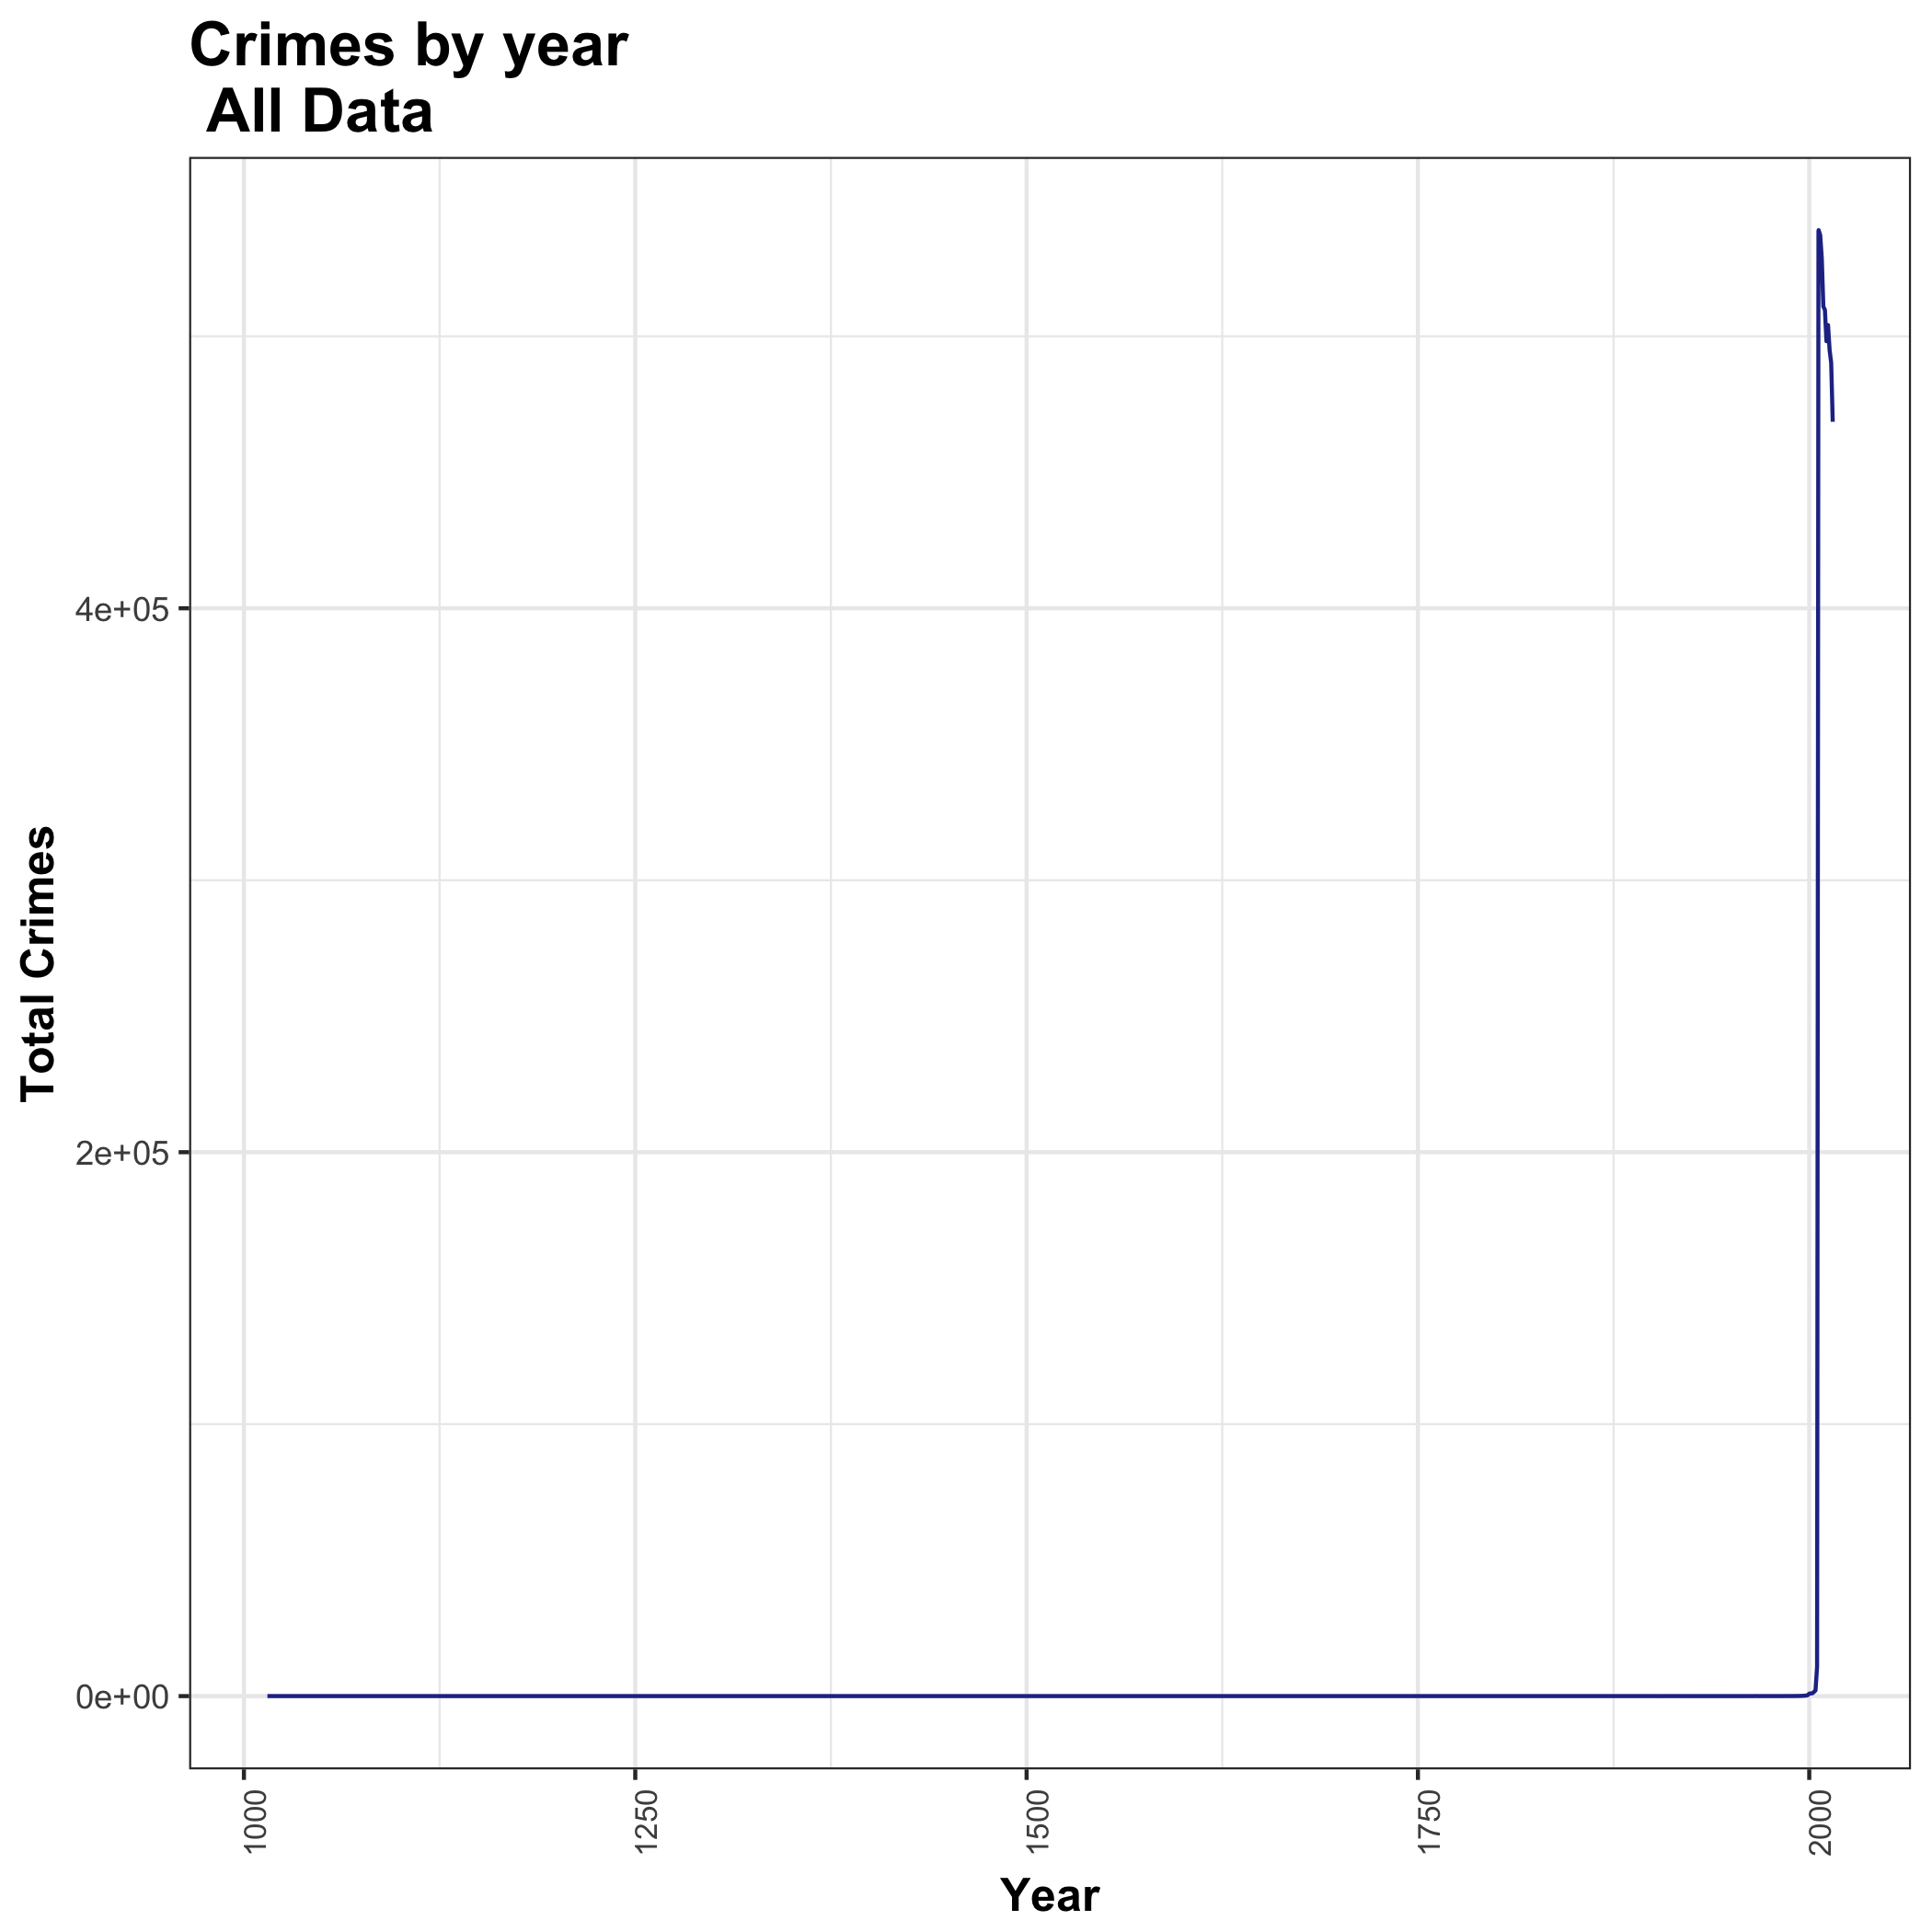
\includegraphics[scale=0.15]{1_YearlyAll.png}
\end{figure}

This plot shows one of the main issues of the data frame: There are 7 observations from the year 1015, a clear invalid value that should be taken out for analysis. But even after keeping all data from year 1990 ownwards, the problem doesn't seem to get better. There is clearly and under-reporting from 1990 until at least 2006, years where the data seems to be captured way after the crime happened. This is even more evident when a Log-scale is applied to Total Crimes, the y-axis.

\begin{figure}[H]
\centering
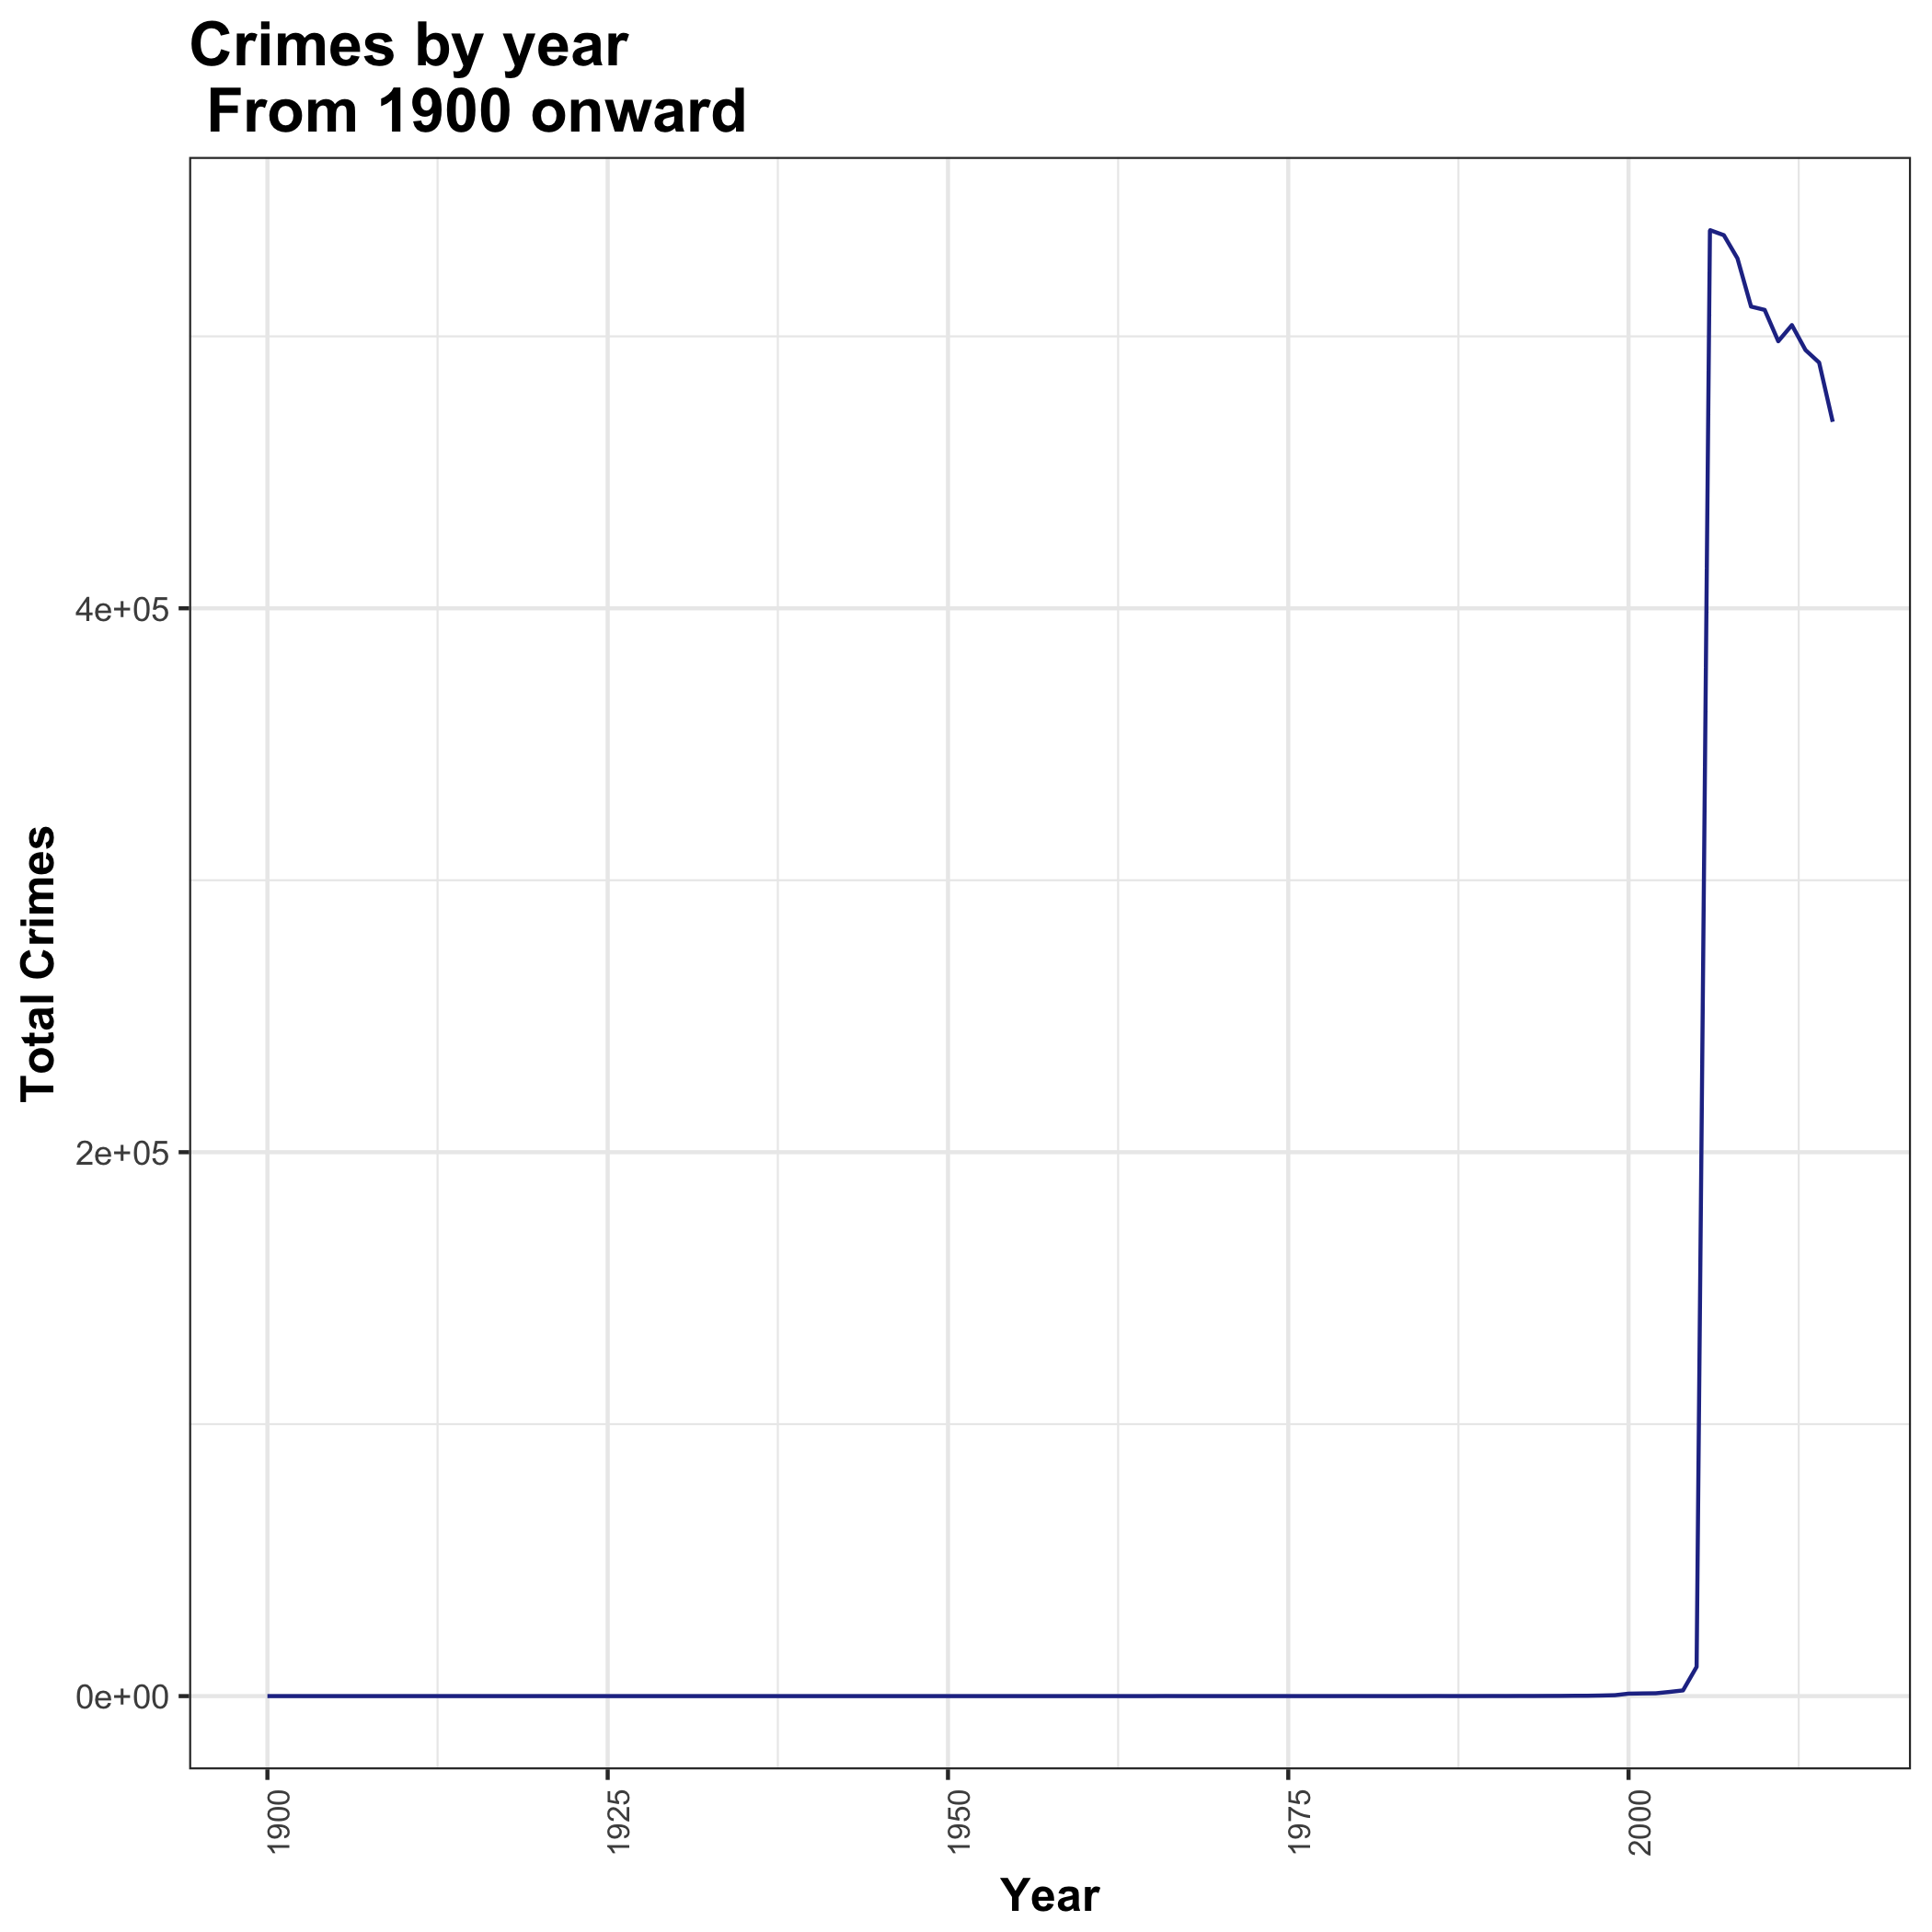
\includegraphics[scale=0.15]{2_YearlyFrom1900.png}
\end{figure}

\begin{figure}[H]
\centering
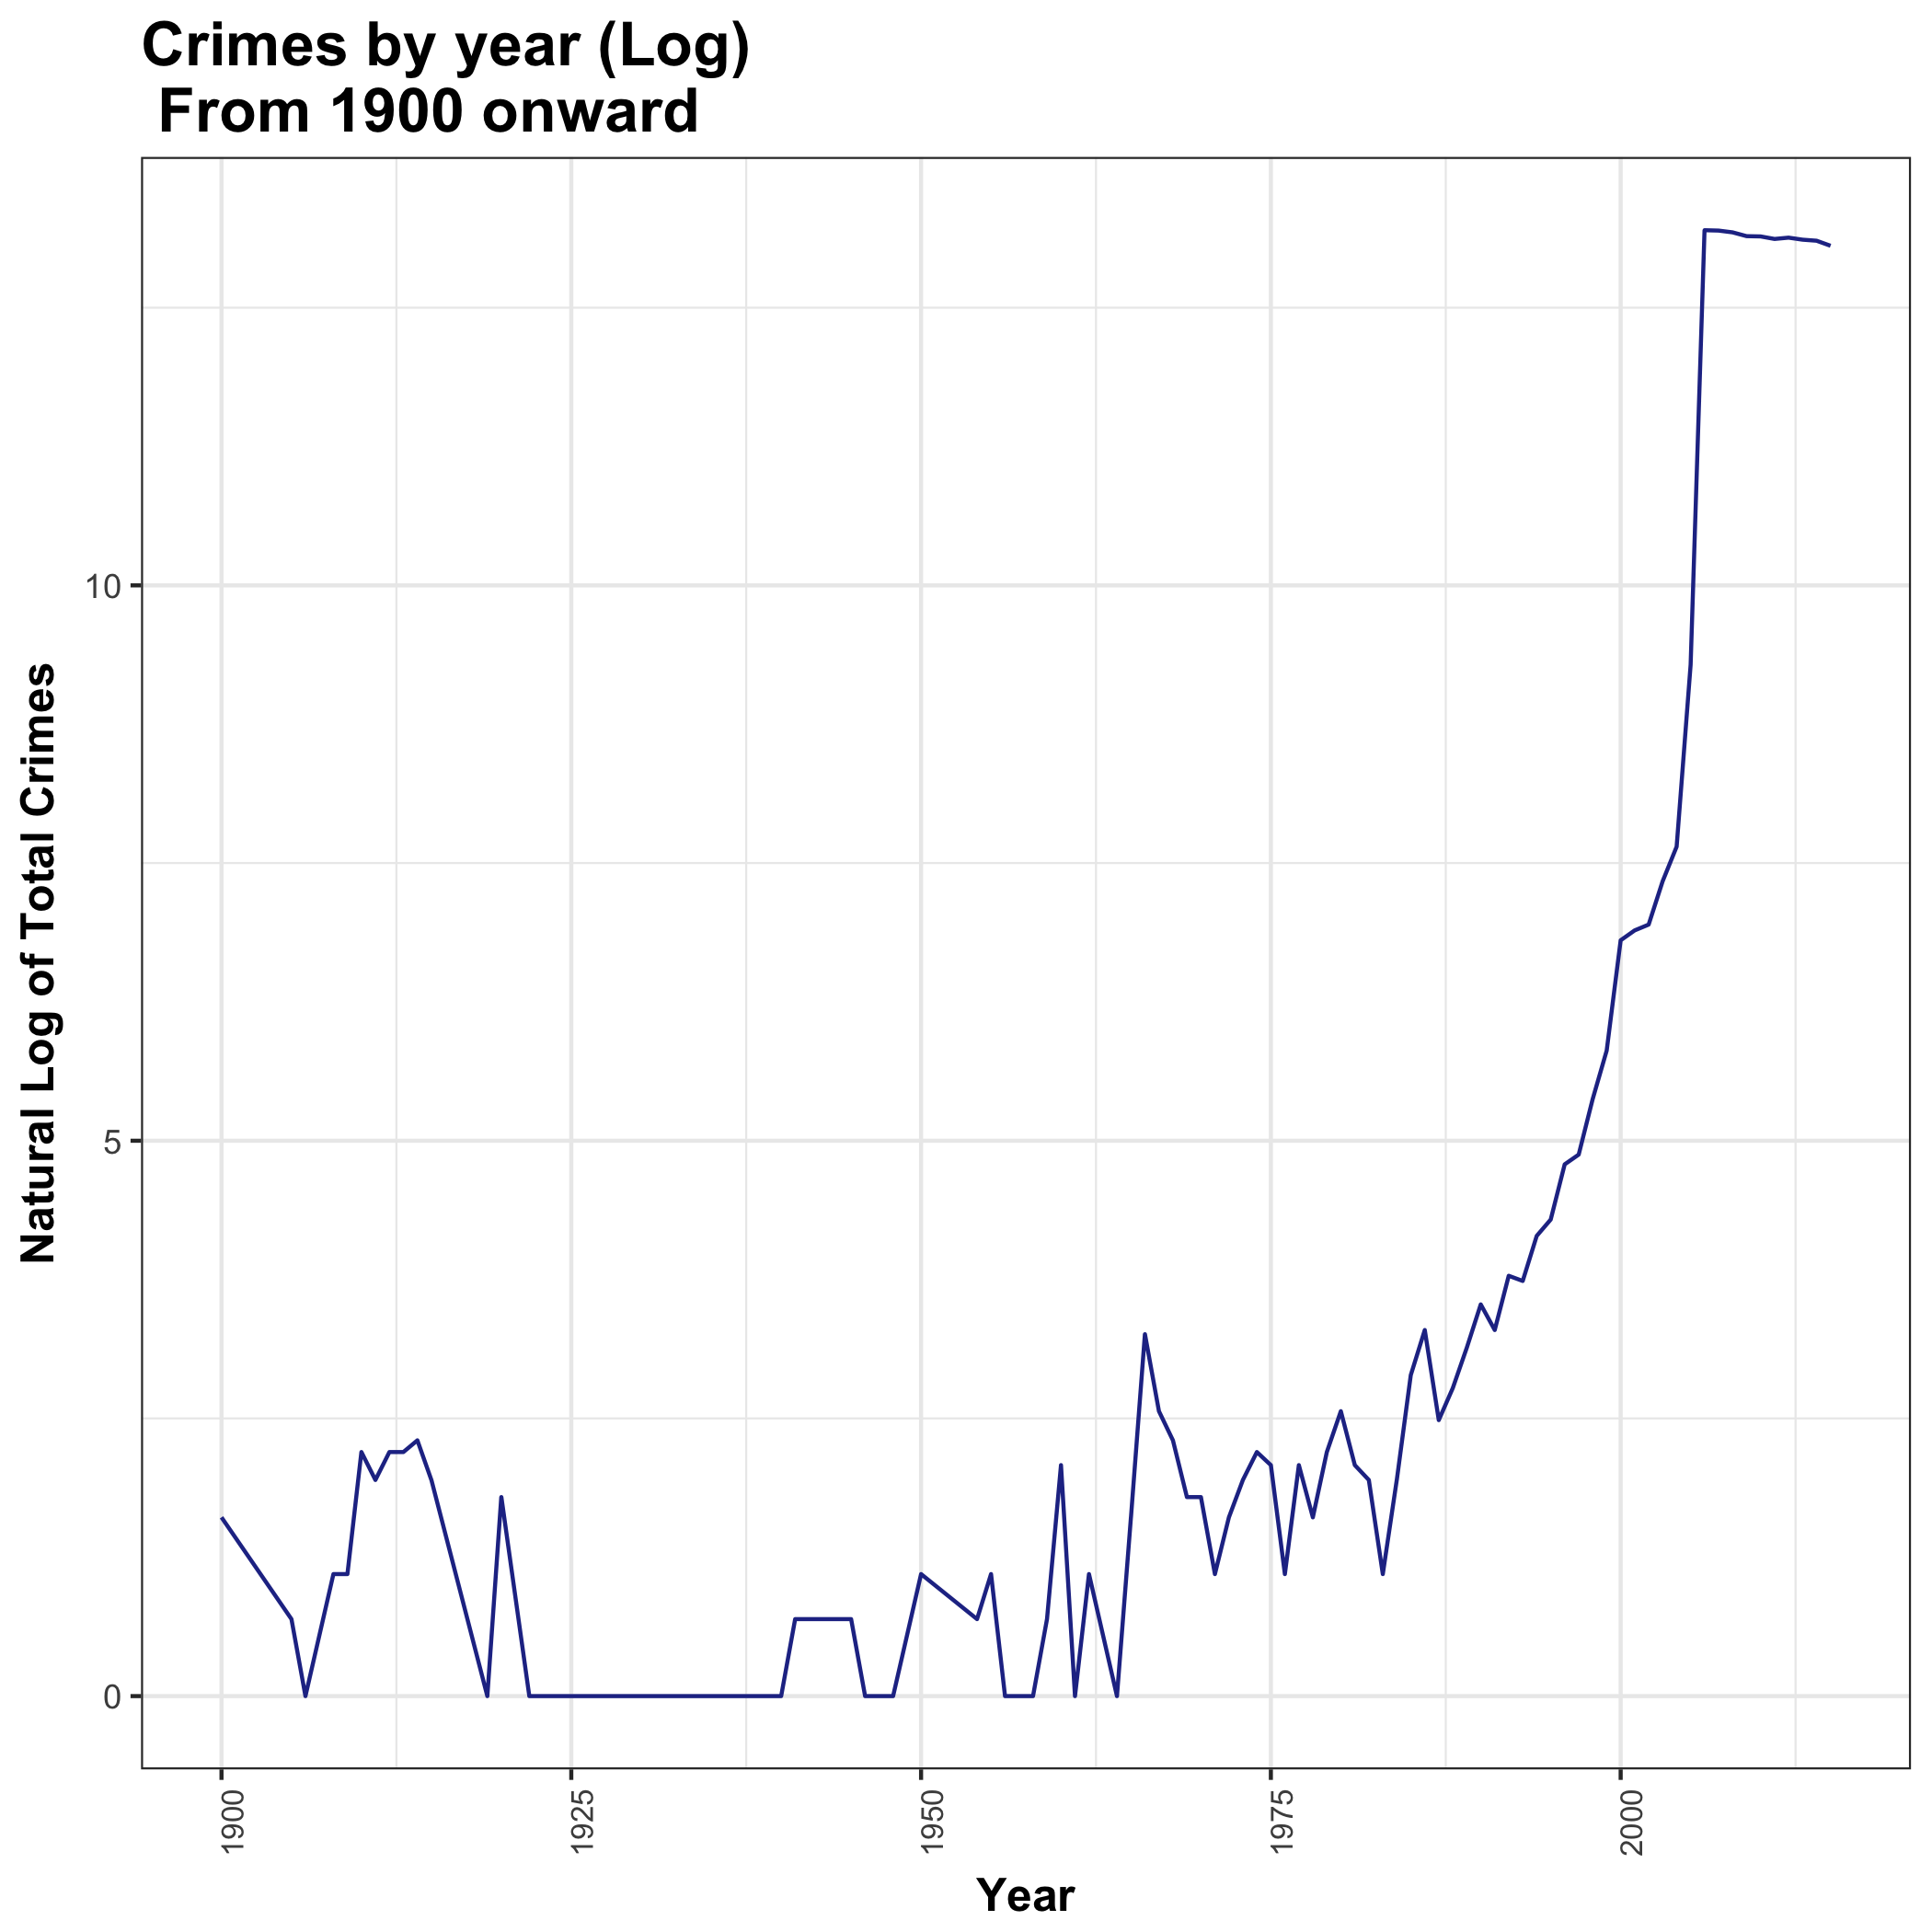
\includegraphics[scale=0.15]{3_LogYearlyFrom1900.png}
\end{figure}

After these, we decided that one issue that was worth inspecting is the difference between year of occurrence (captured in \texttt{CMPLNT\_FR\_DT}) and year of reporting (from the column \texttt{RPT\_DT}. The instability of this measure is staggering when we consider all years of occurrence after 1900.   

\begin{figure}[H]
\centering
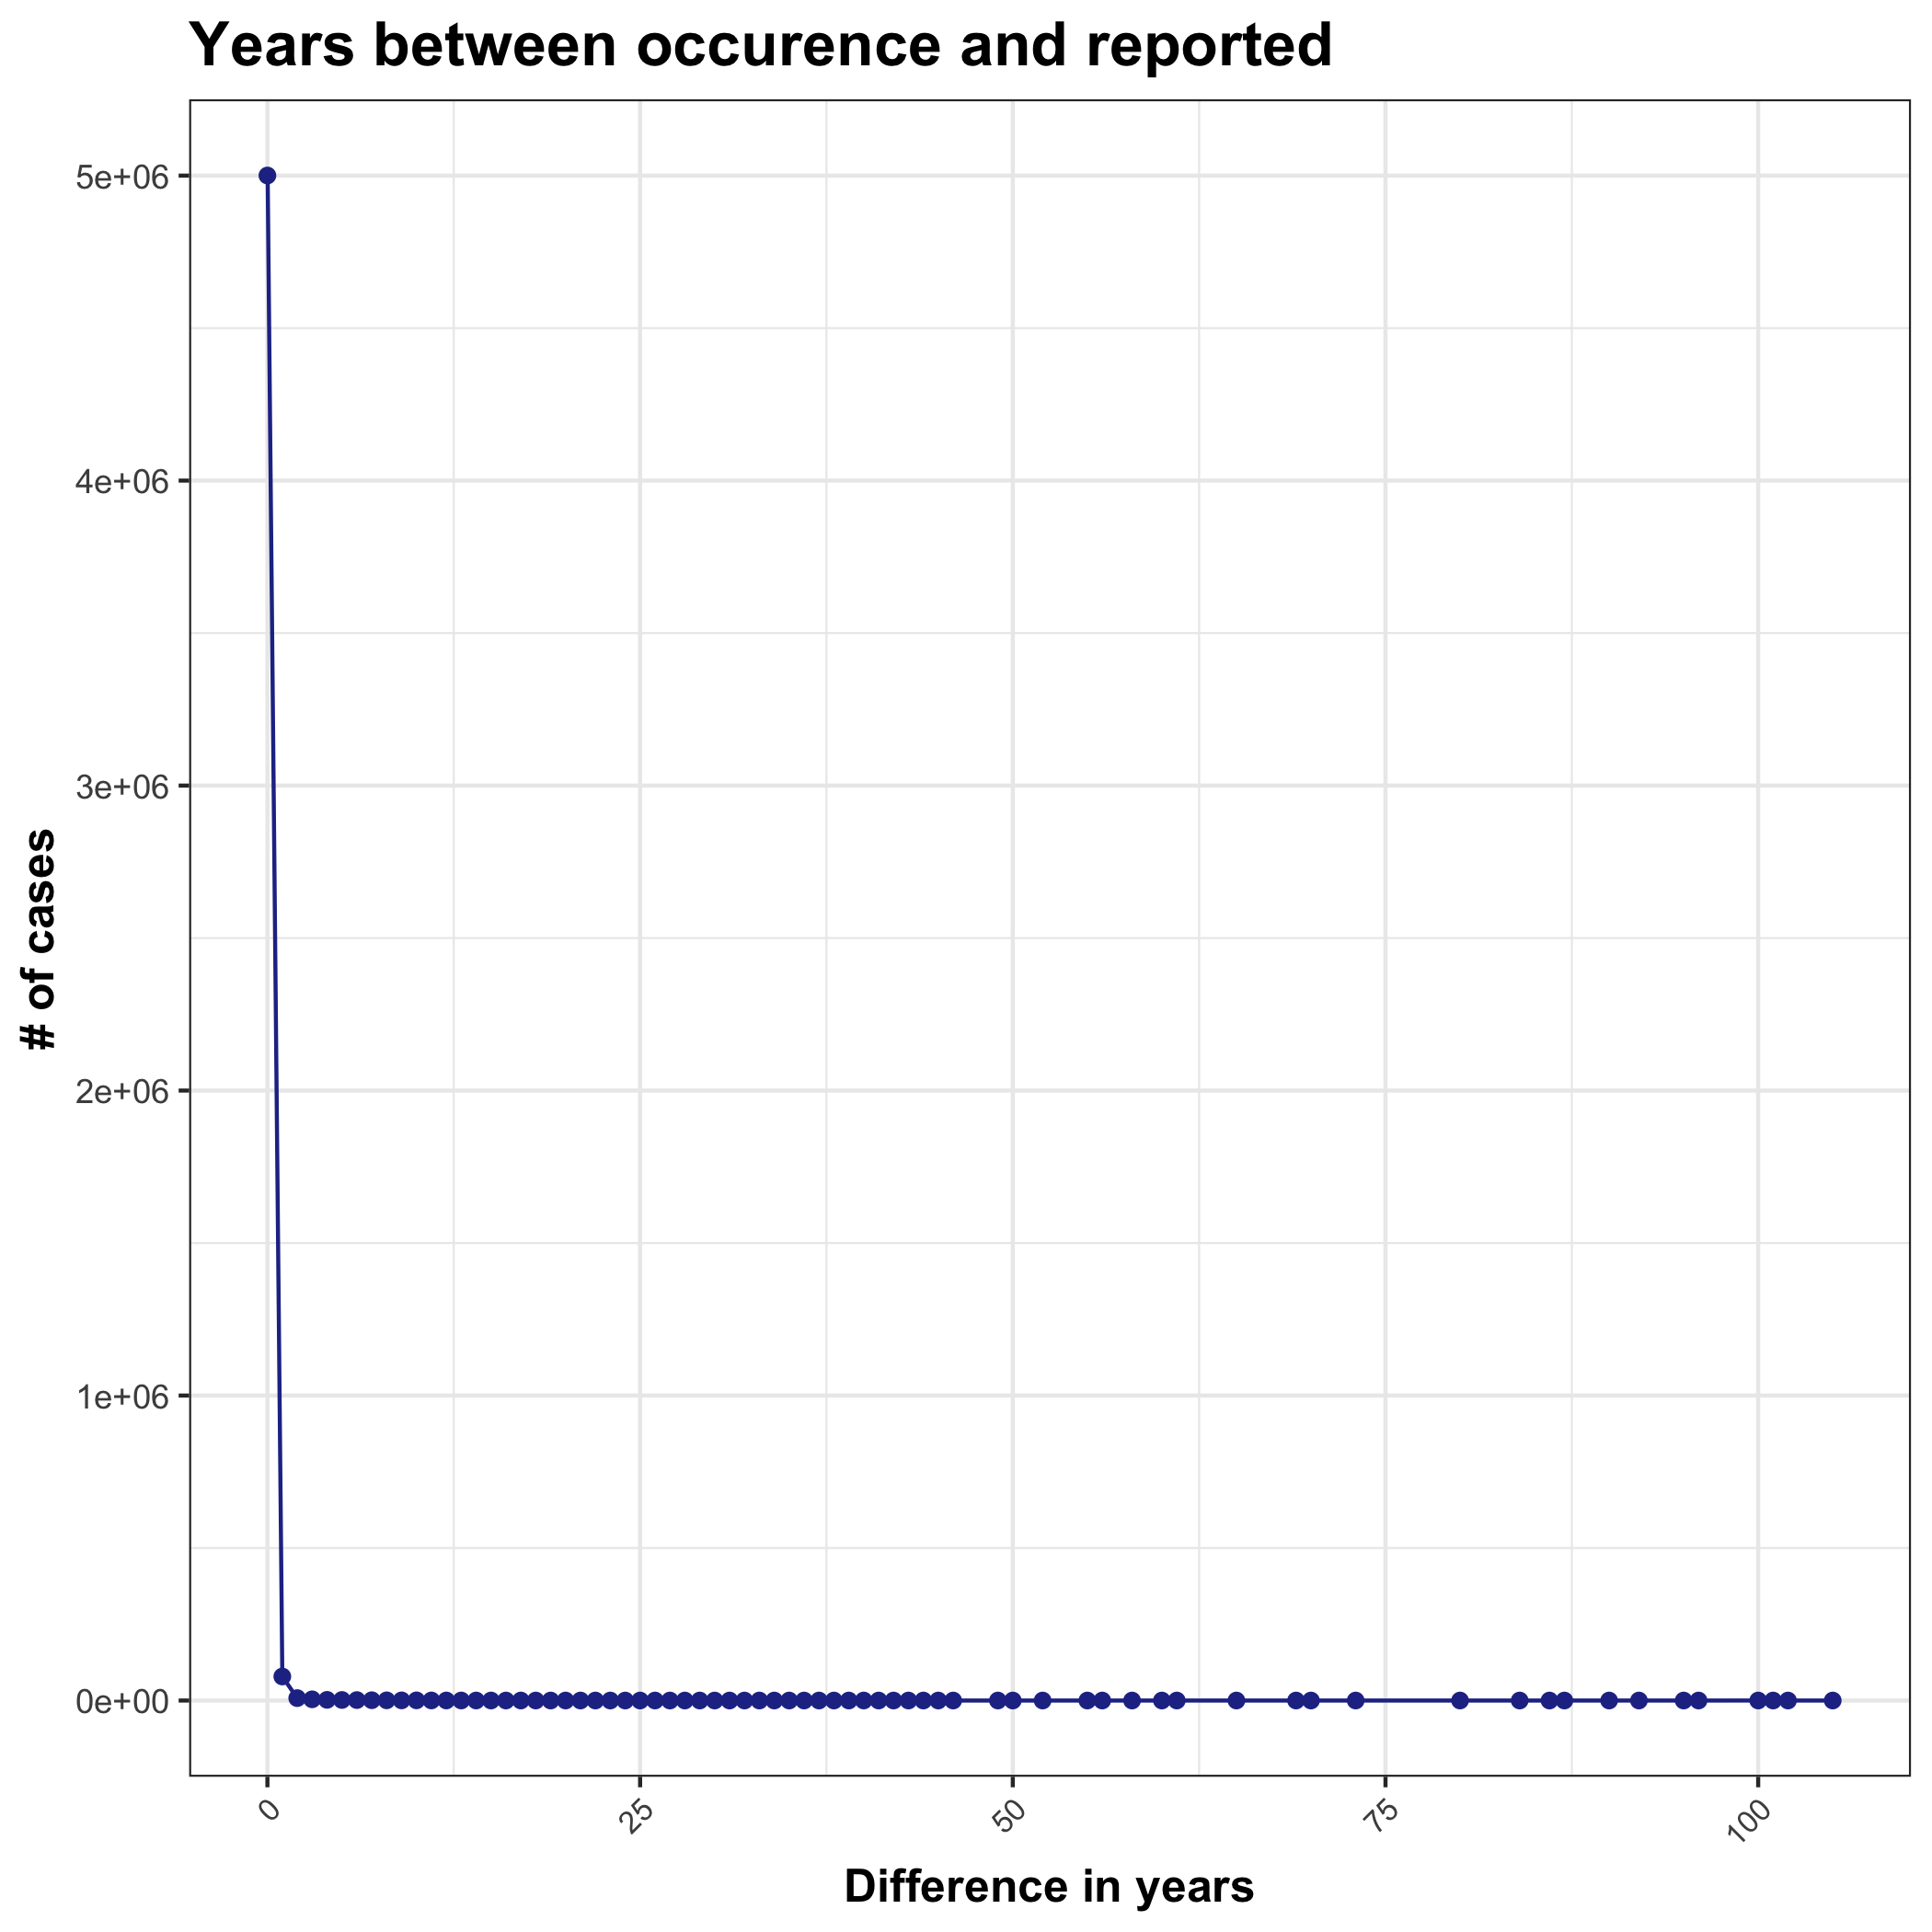
\includegraphics[scale=0.14]{8_DiffYears.png}
\end{figure}

\begin{figure}[H]
\centering
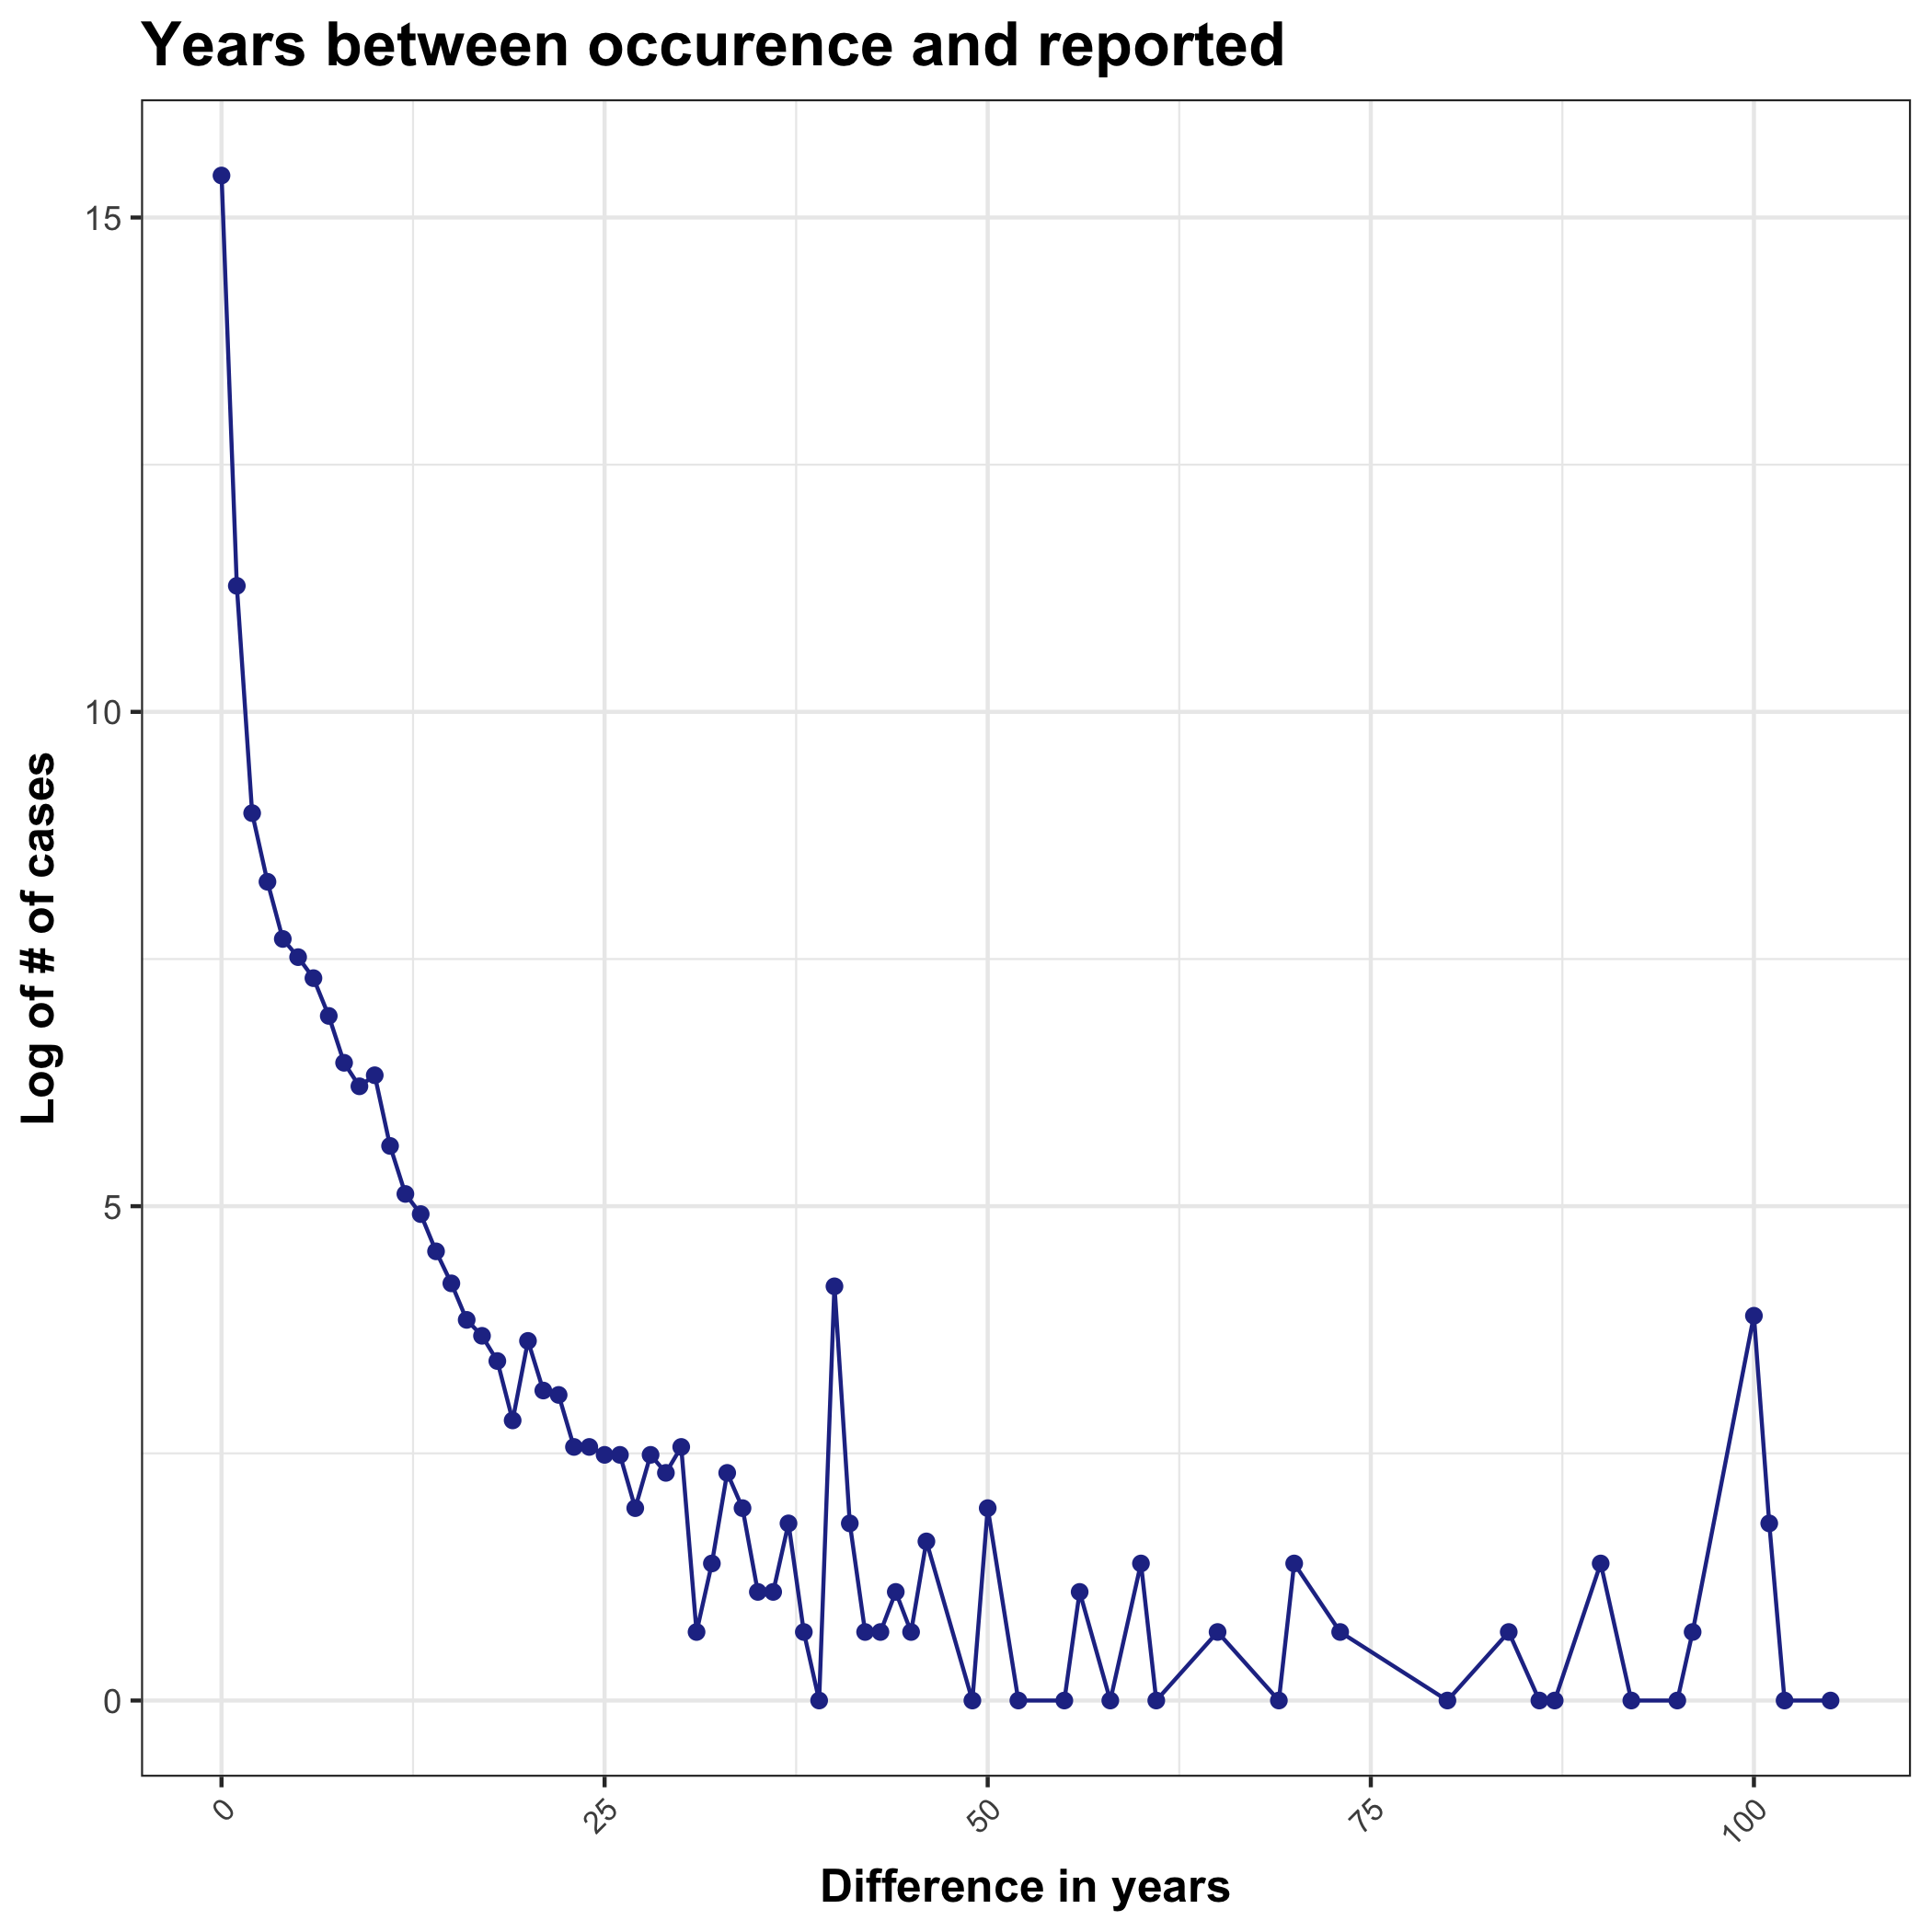
\includegraphics[scale=0.14]{9_LogDiffYears.png}
\end{figure}

Although most of the crimes are reported on the same year (98\% of all data) or the year after (1.5\%, probably due to crimes in December and reported on January next year), there are a large number of crimes with huge difference between the year it was reported and committed. For example, there are 49 crimes with a difference of 100 years between occurrence and reporting. By seeing the data, we can almost confirm, for example, that these cases have been miscoded for year of occurrence: 

\begin{center}
\textbf{Cases with 100 years of difference between occurrence and reporting} \\
\begin{tabular}{ |c|c|c| } 
\hline
\textbf{Year occurrence} & \textbf{Year reported}  & \textbf{Number of cases} \\
\hline
   1909 & 2009 & 1 \\ 
   1912 & 2012 & 9 \\ 
   1910 & 2010 & 7 \\  
   1913 & 2013 & 7 \\  
   1914 & 2014 & 9 \\ 
   1906 & 2006 & 1 \\ 
   1915 & 2015 & 7 \\ 
   1911 & 2011 & 6\\ 
   1908 & 2008 & 3 \\ 
\hline
\end{tabular}
\end{center}

The question then is: Should we recod this cases? Add 100 years to them? Or simply discard them? To answer this question, let us first do the same plots as above, but only with the years 2006 ownwards: 

\begin{figure}[H]
\centering
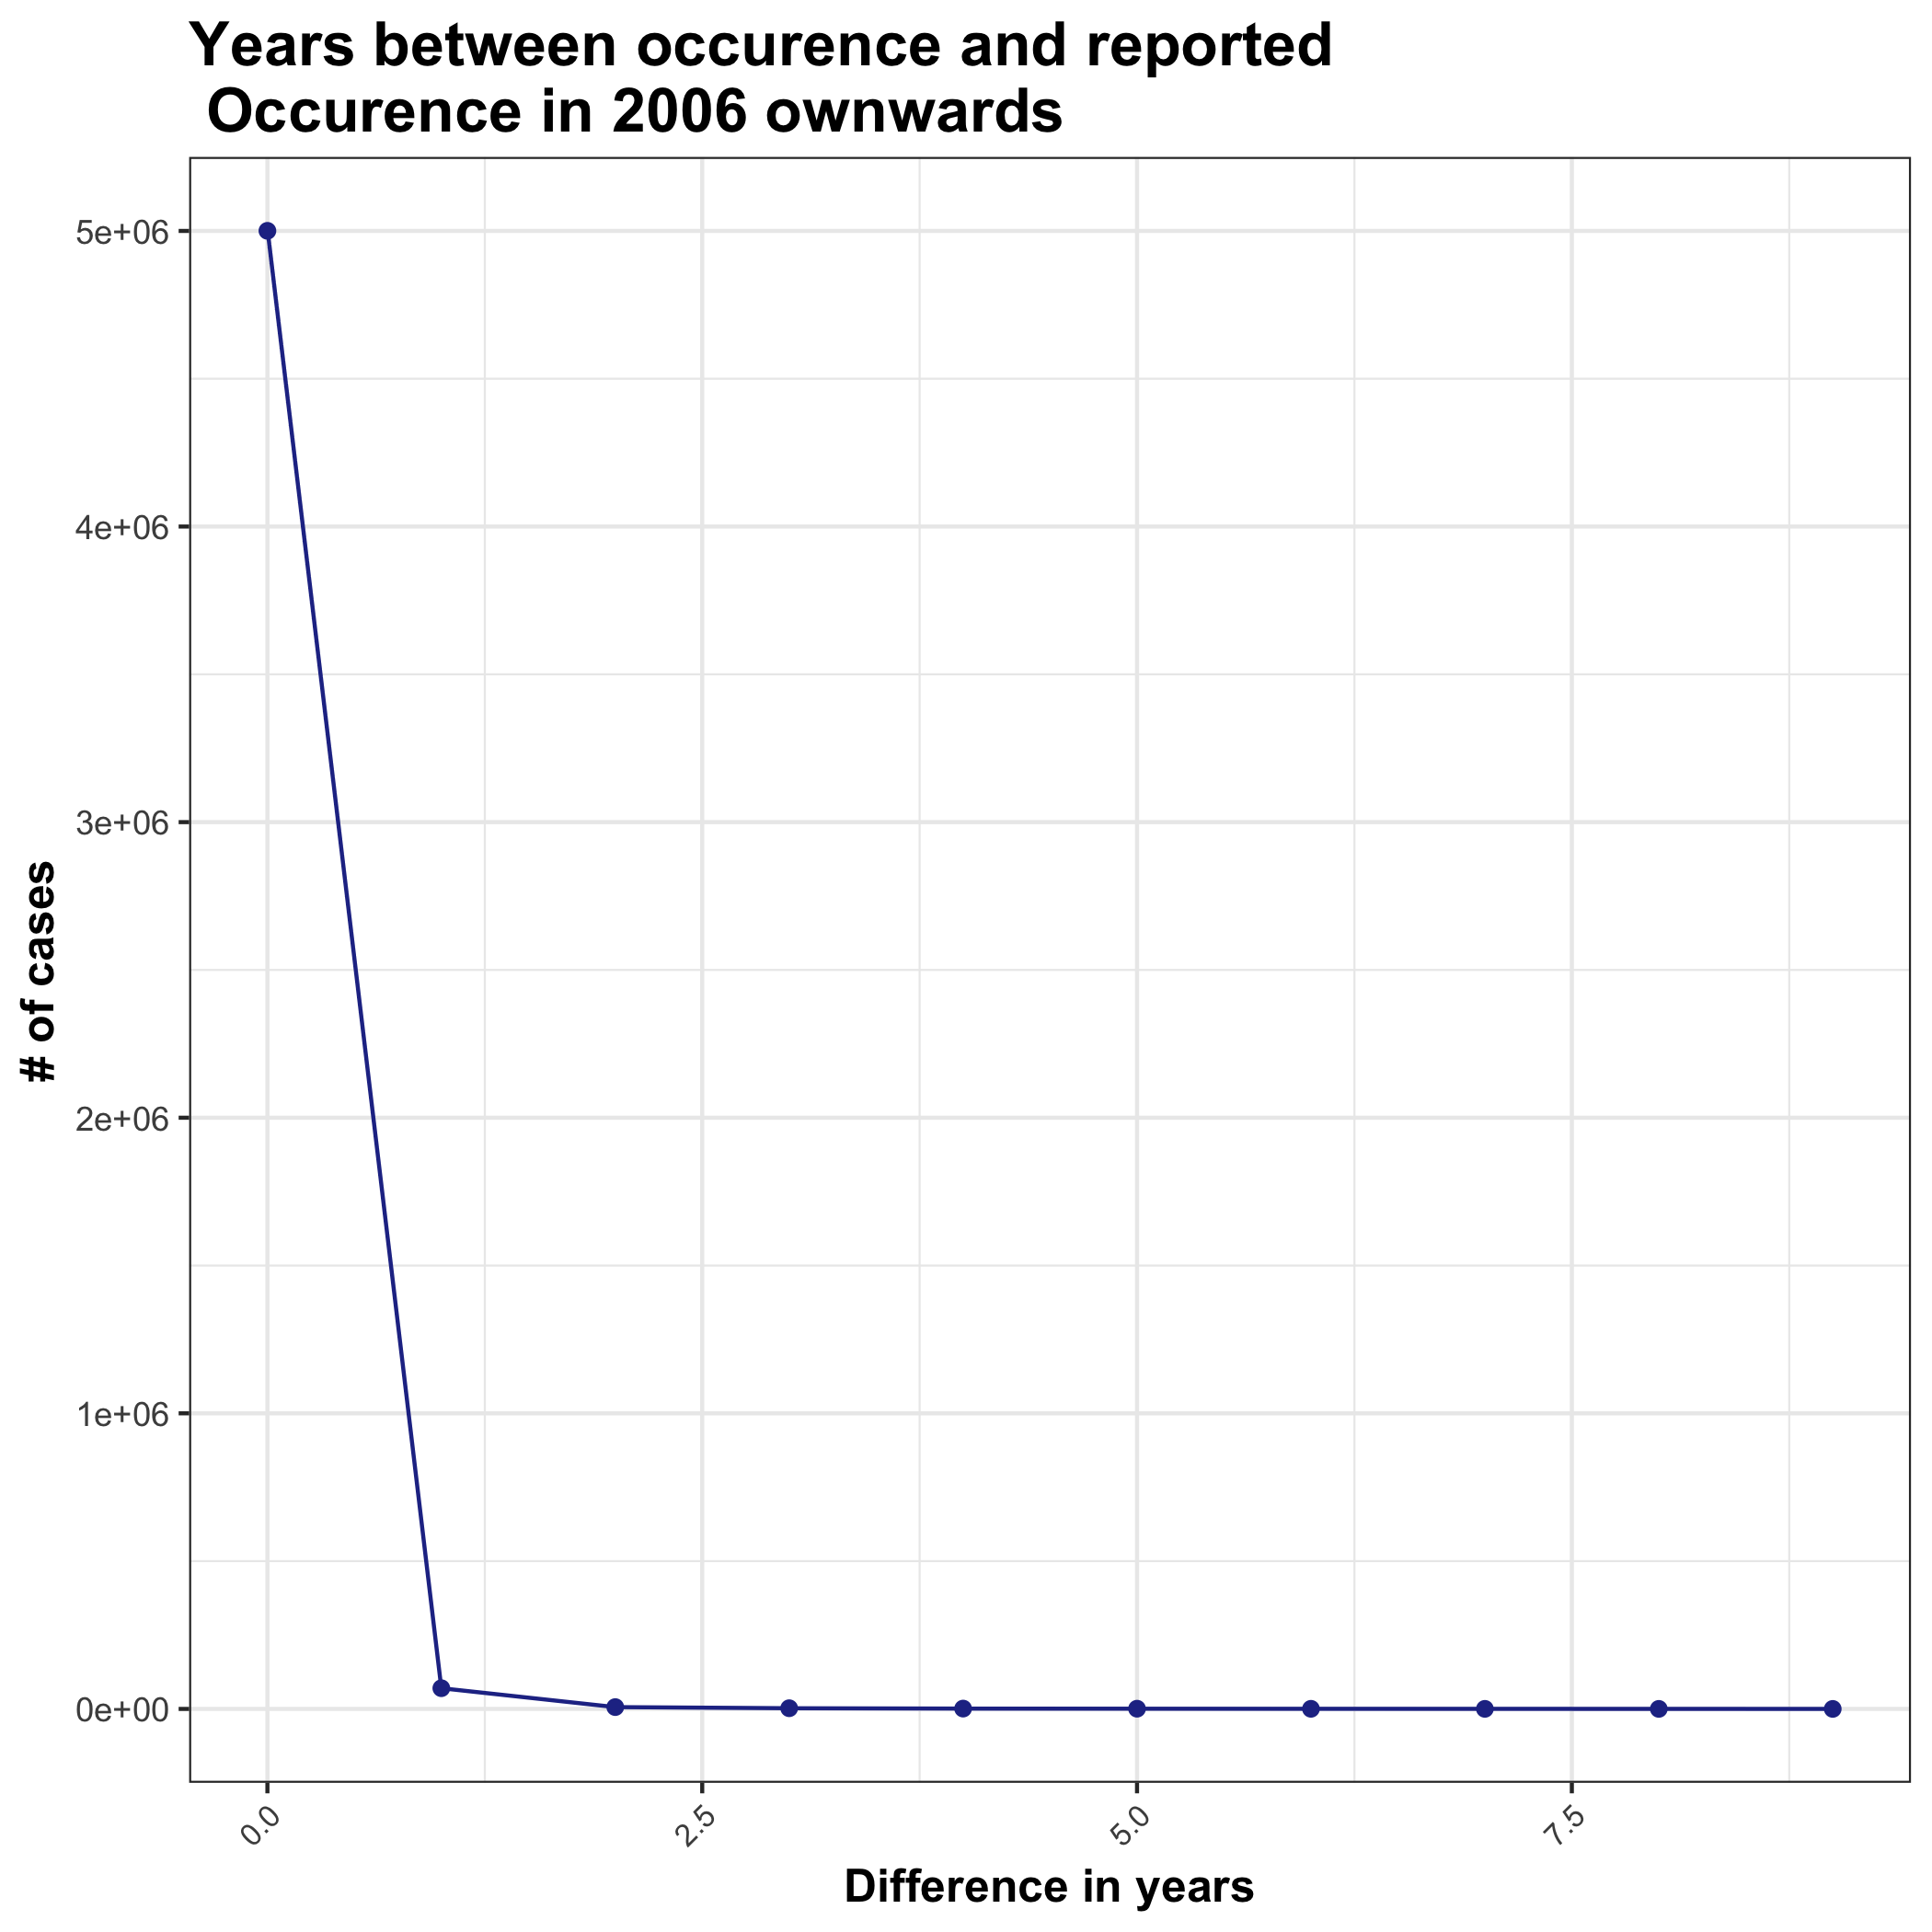
\includegraphics[scale=0.14]{10_DiffYears_2006.png}
\end{figure}

\begin{figure}[H]
\centering
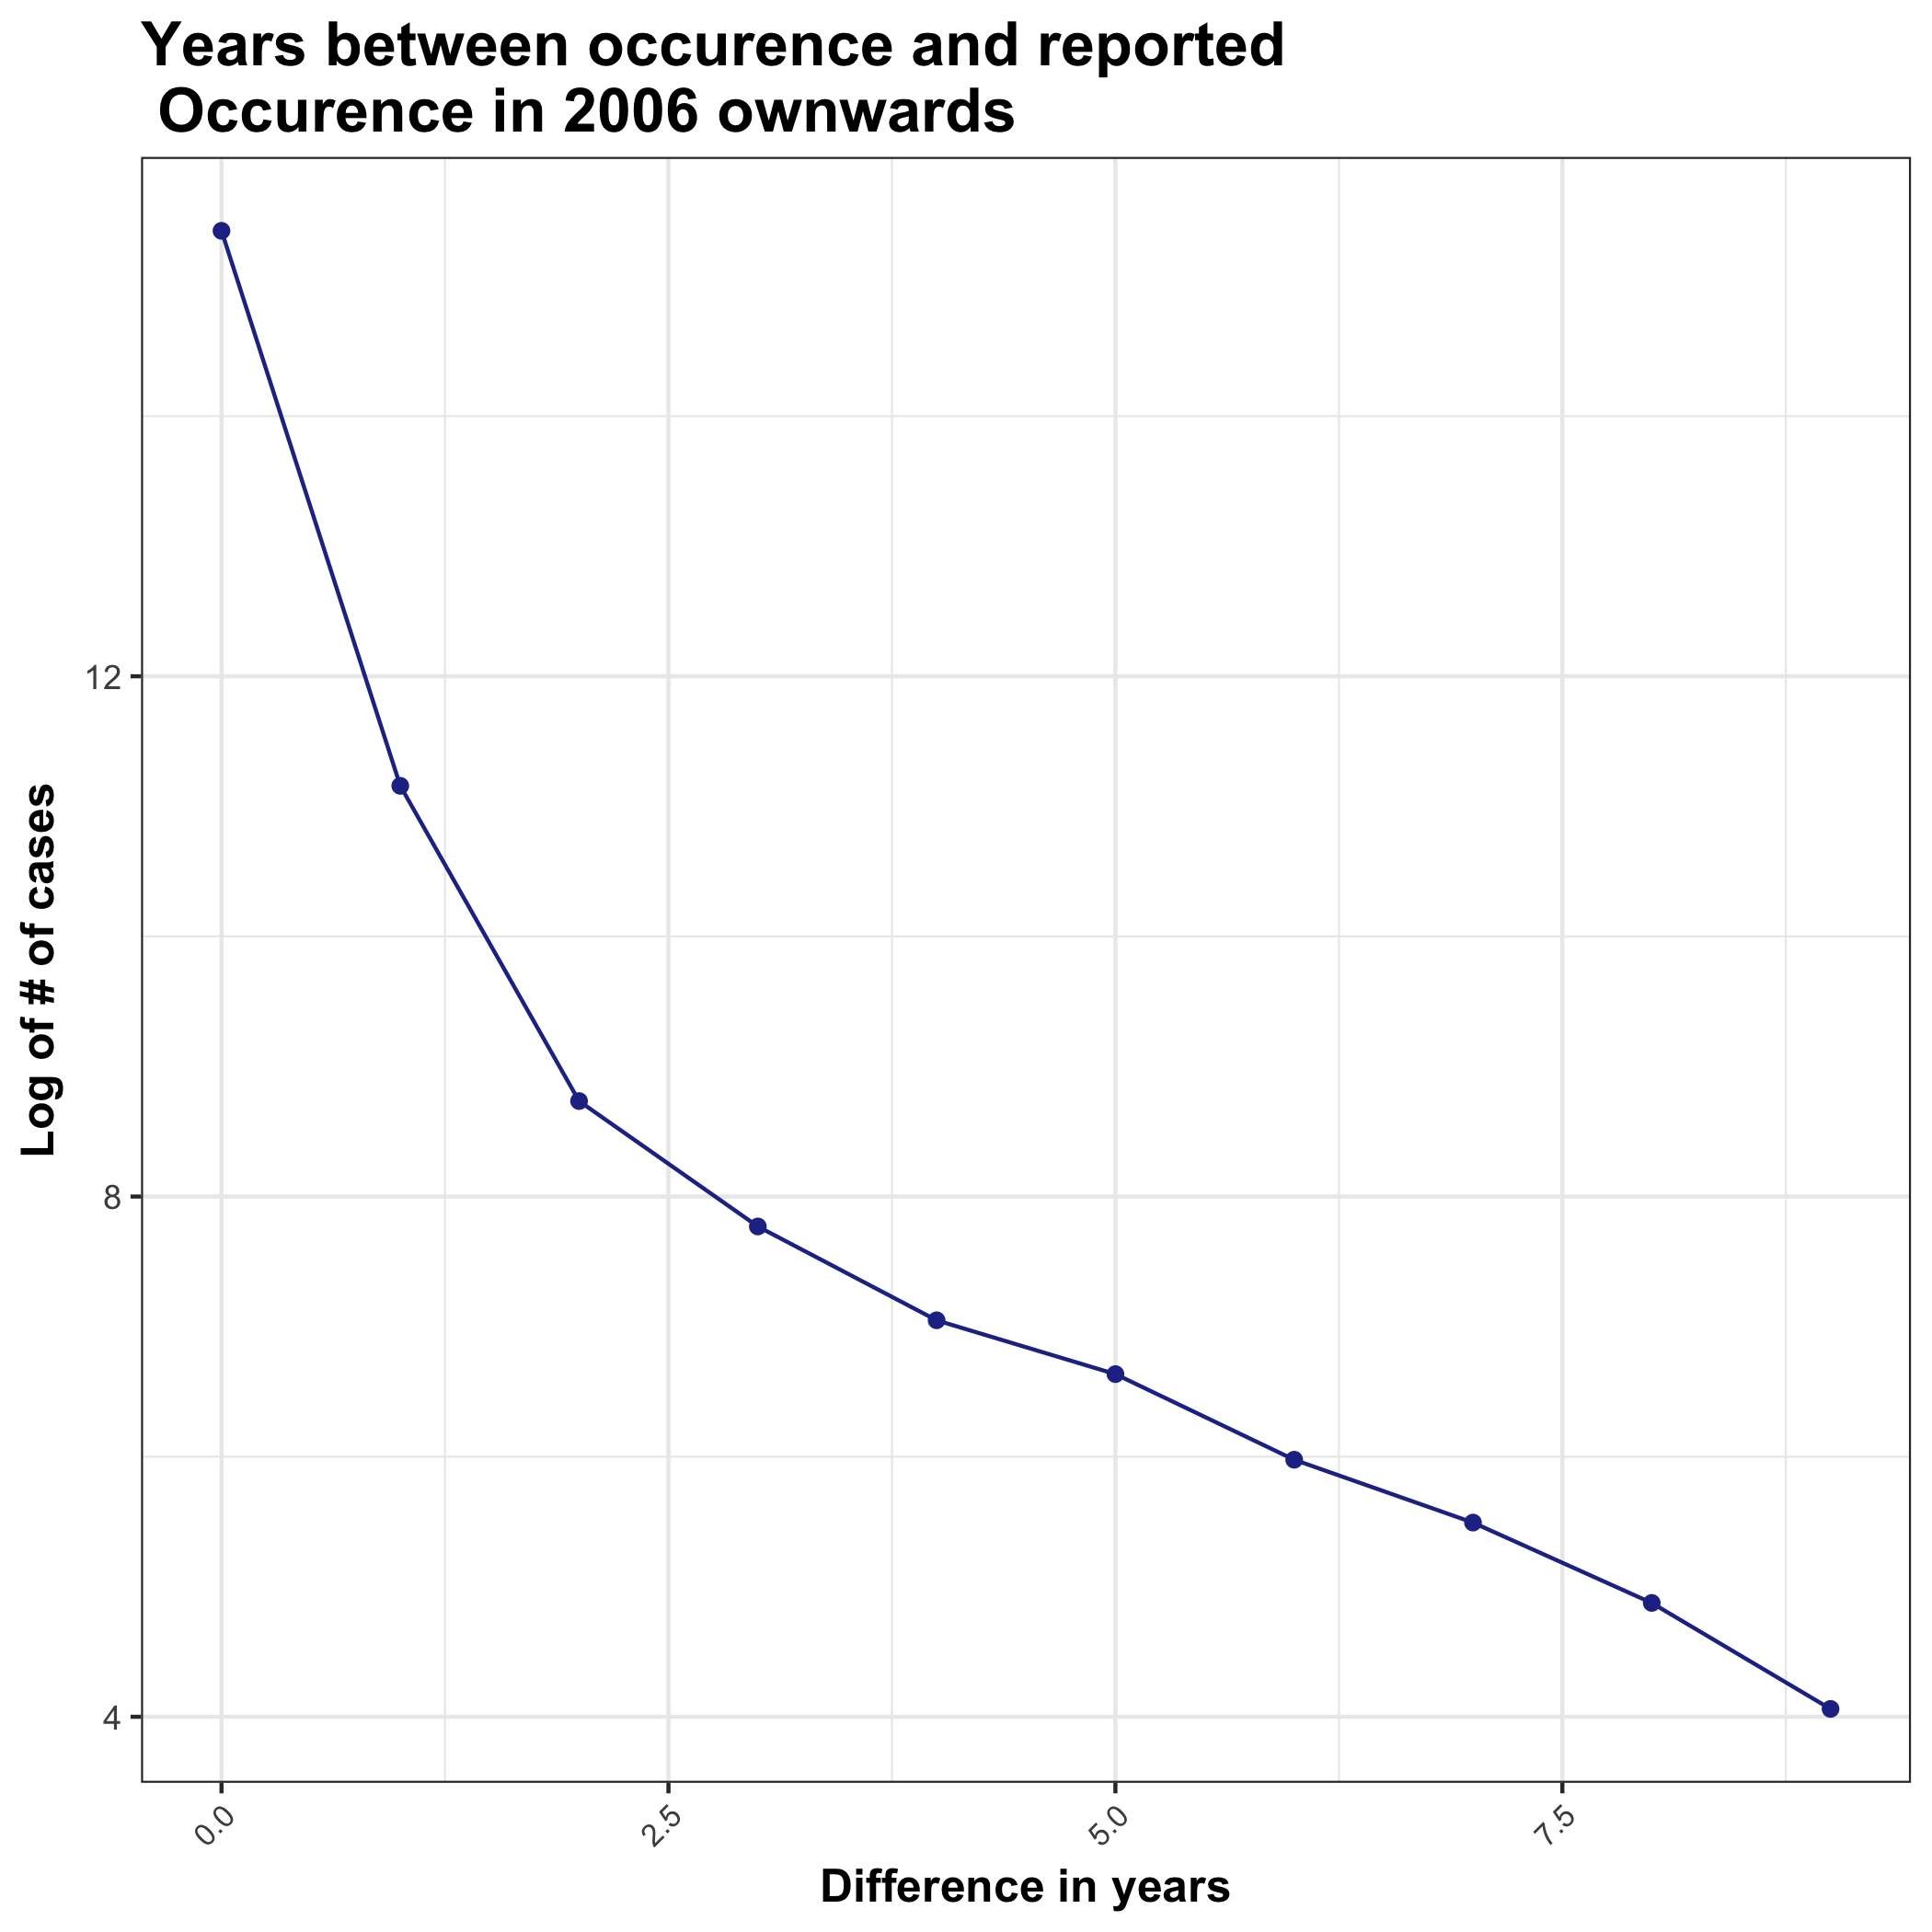
\includegraphics[scale=0.14]{11_LogDiffYears_2006.png}
\end{figure}

In this case, we can see what it looks like a natural and more steady line of descent between year of reporting and year of occurence. This, it is our believe, are valid cases: Some crimes just take a long time to be reported, maybe because of the victim is simply traumatized, or maybe because there are crimes that can las for years. In any case, it looks to us that the best strategy for the analytic section is going to be to keep only the cases that have a year of occurrence from 2006 onwards, and in fact discarding the cases that have been miscoded for year. 

That being said, we continued with a similar analysis with the time of occurrence. At first, we decided to plot all the crimes by hour, to see if there were any differences by time of the day. As seen below, it's clear that most crimes are registered by the exact hour, but few have information about the exact minute when it was registered. 

\begin{figure}[H]
\centering
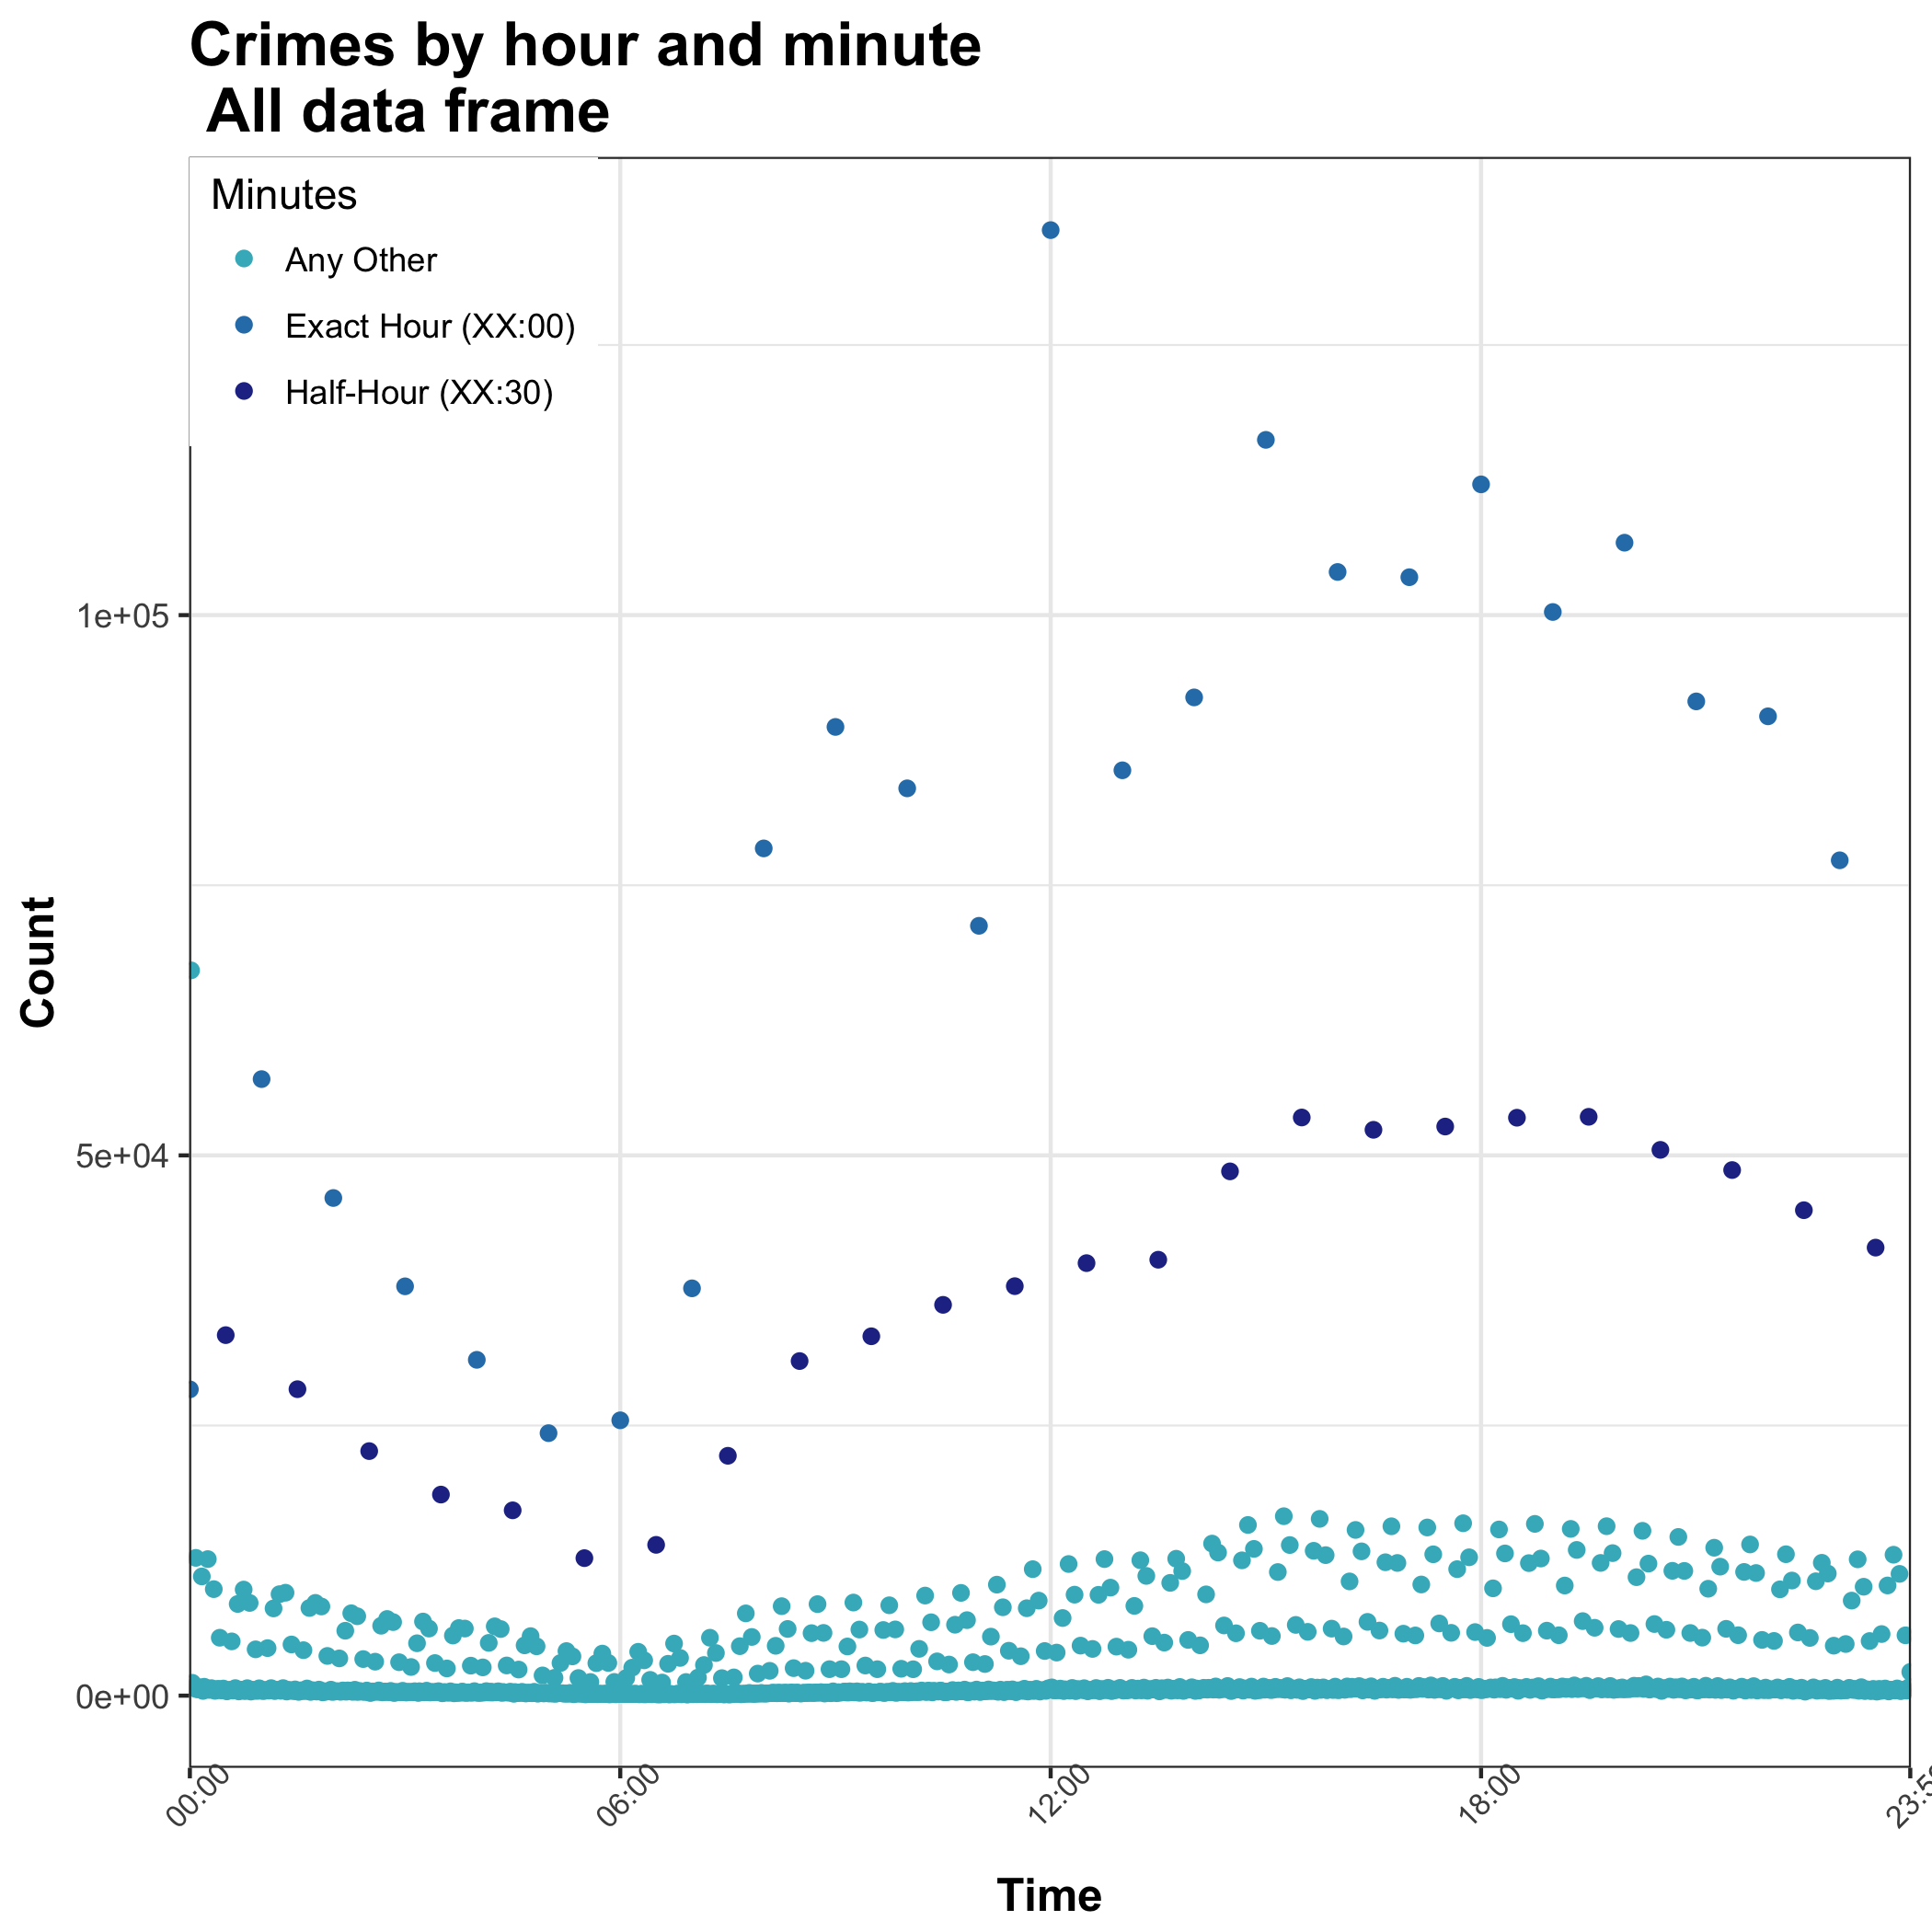
\includegraphics[scale=0.15]{4_HourMinute.png}
\end{figure}

To fix this and observe tendencies by time of the day, we decided to round the minutes to the hour (i.e., if a crime was registered at 6:01 or at 6:59, we consider it to be at 6:00). This lets us observe the tendency of crimes. Clearly, most of the crimes are committed between 3:00 pm and 8:00 pm. The following graph also shows us an issue: There is a slight spike when it comes to 12:00. Probably, many crimes when the time is not registered are encoded automatically to noon. 

\begin{figure}[H]
\centering
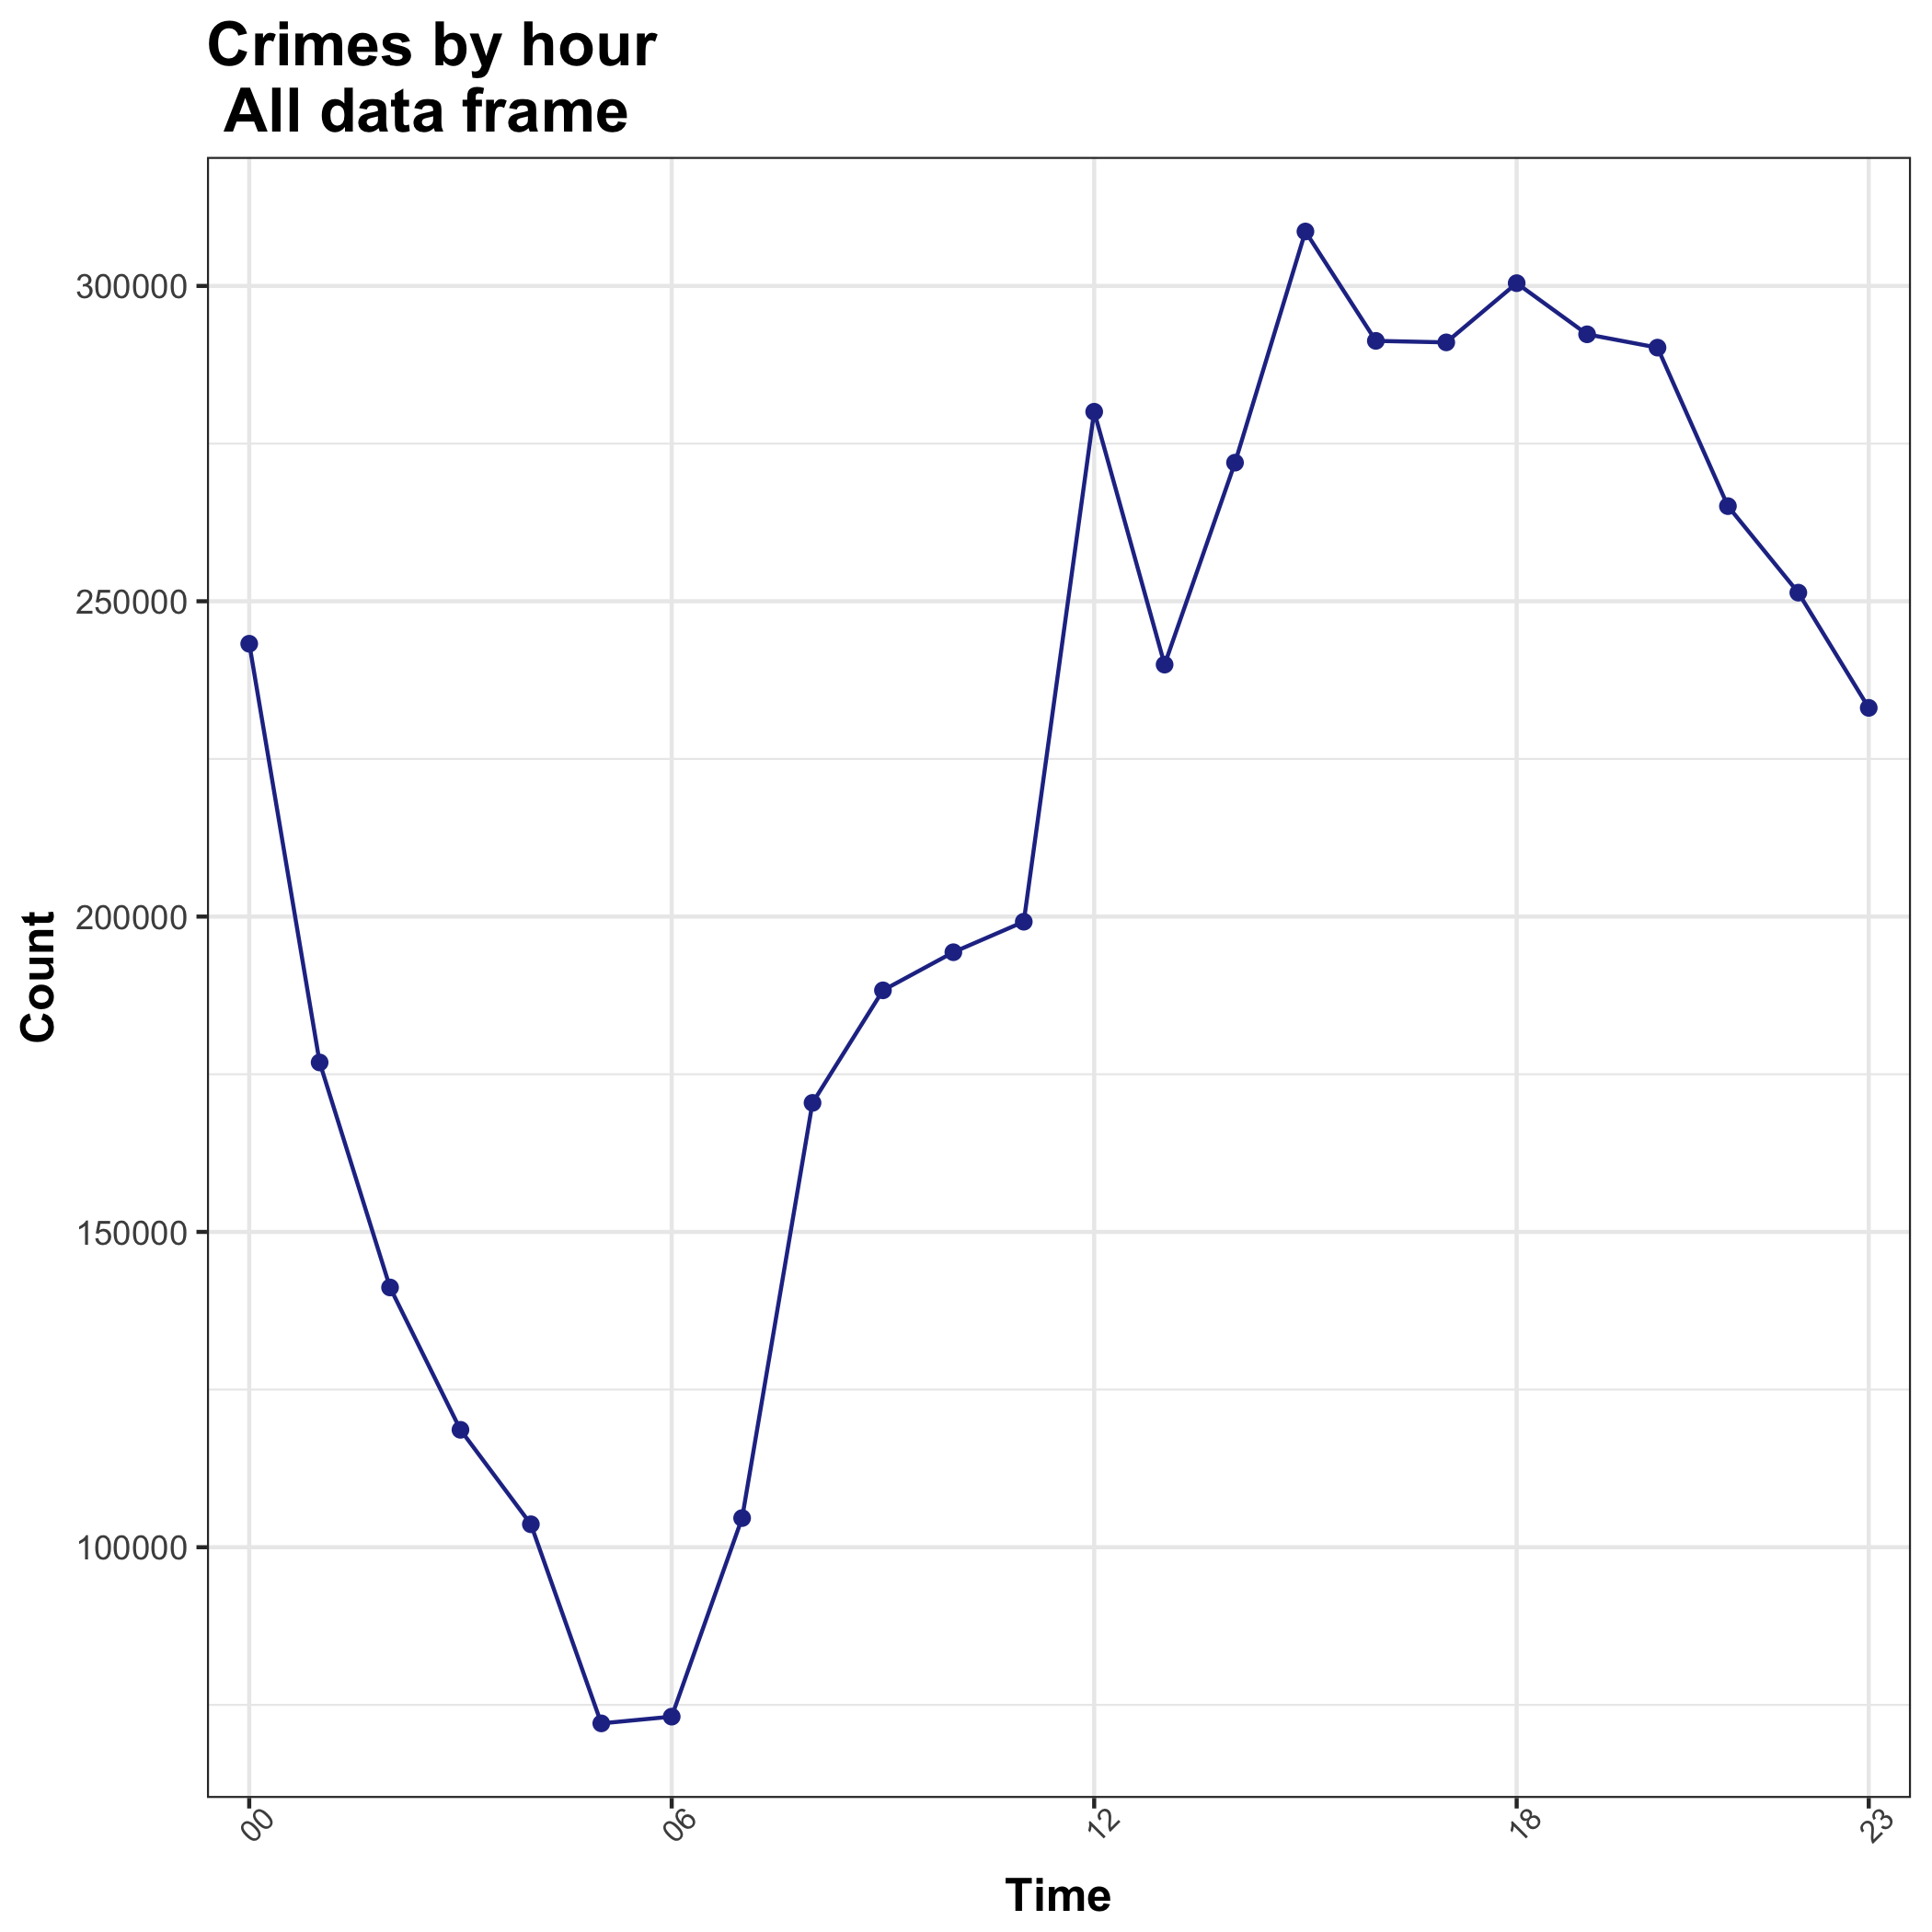
\includegraphics[scale=0.15]{5_Hour.png}
\end{figure}

Finally, we did a  a quick analysis by the type of crime, encoded in the column \texttt{OFNS\_DESC}. Before begin describing the main findings, it's worth noticing that the variables\texttt{KY\_CD} and \texttt{OFNS\_DESC} do not match one to one. For example, "abortion" has more than one code assigned to it. This, as it was stated above, could easily by analyzed if an external codebook for Crime ID was published. 

In any case, we took all the crimes from 2006 to make an analysis of the most common type of crimes in New York City. From this year on, there are 18,775 with no type. Out of 5081794 (this is, 0.36\% of the data). Some categories, like the crime for "Fortune Telling" has only one observation, a crime apparently committed in 2015. The 6 main categories add a total of 3,222,141 crimes, representing  63.64\% of the data. Murder ("MURDER \& NON-NEGL. MANSLAUGHTER"), on the other hand, has only 4444 cases from 2006, barely 0.008\% of the crimes committed in NYC. Rape, another crime that might be of particular interest, has 12,986 cases on the data frame, and Sex Crimes (we assume, other that rape), 53,213 cases. 

We also decided to perform a quick analysis of the 6 main crimes in NYC over 2006 - 2015. From this, only "Dangerous Drugs" seem to have a negative trend over time: From 2006 to 2015, the crimes for this category went from 36126 to 23645, a reduction of 34.5\%. Other crimes, as HARRASSMENT, seem to have declined until 2013, to see later a spike towards 2014 and 2015. 


\begin{figure}[H]
\centering
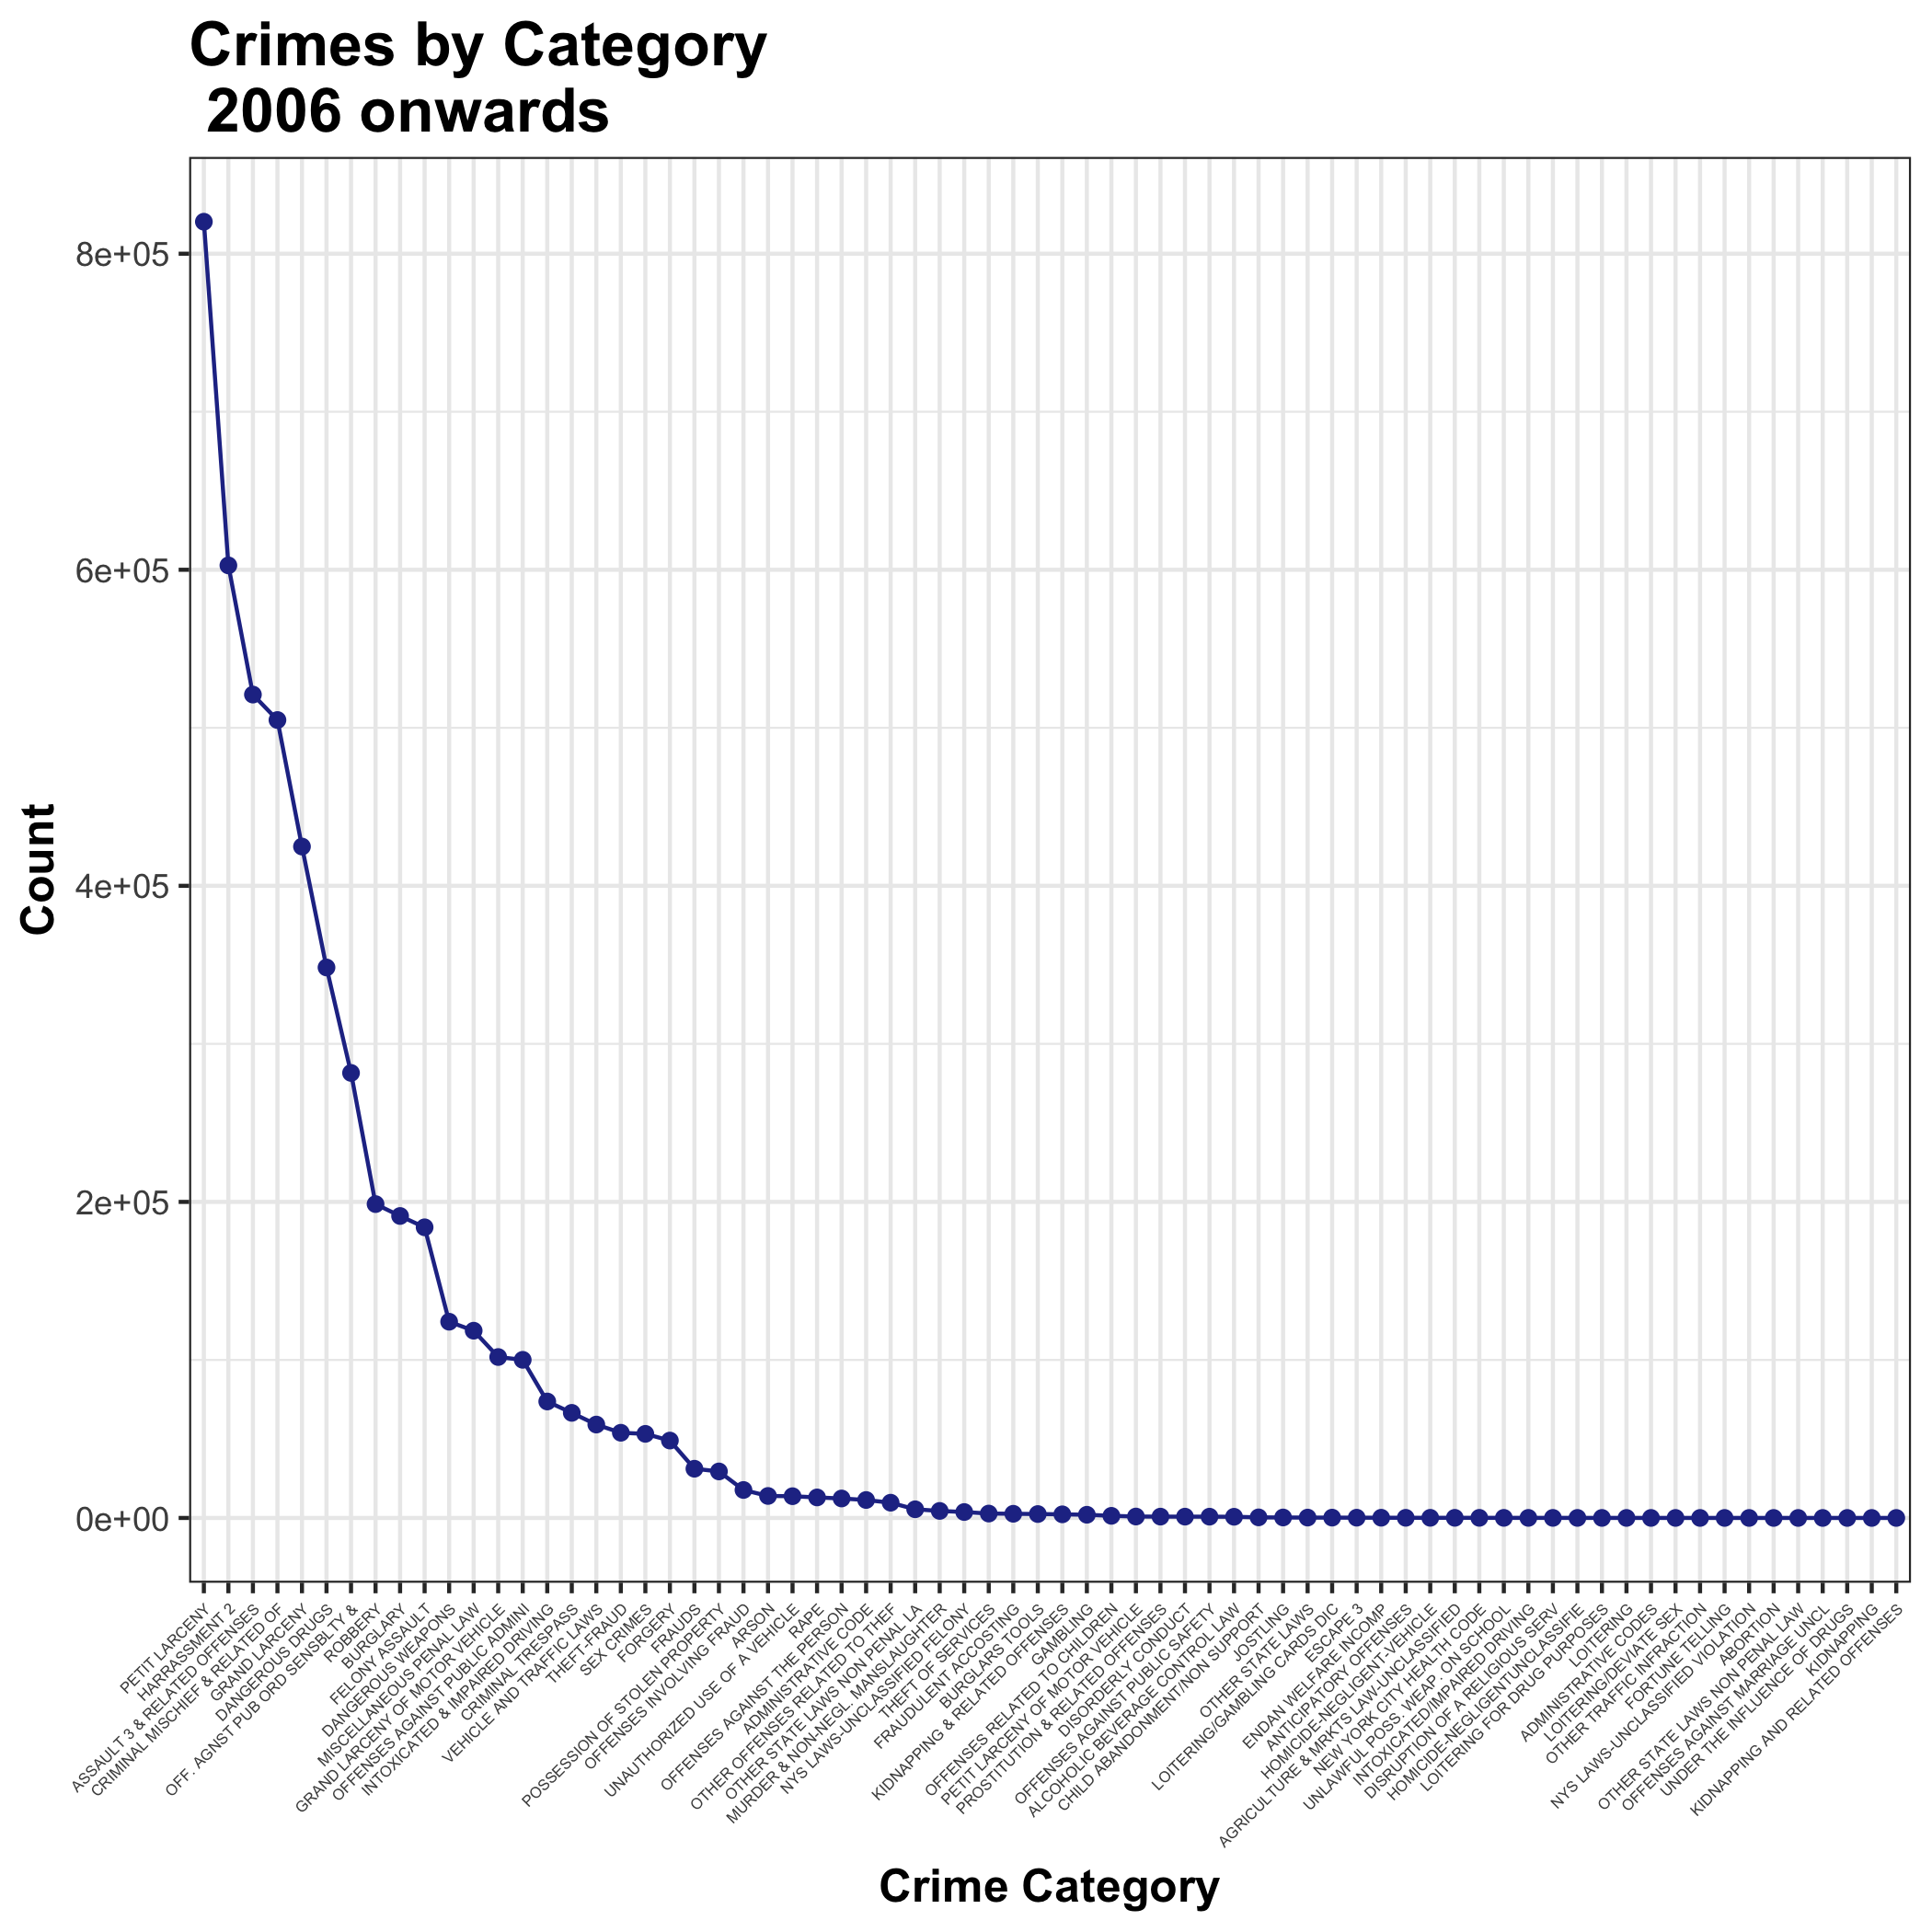
\includegraphics[scale=0.16]{6_Type.png}
\end{figure}

\begin{figure}[H]
\centering
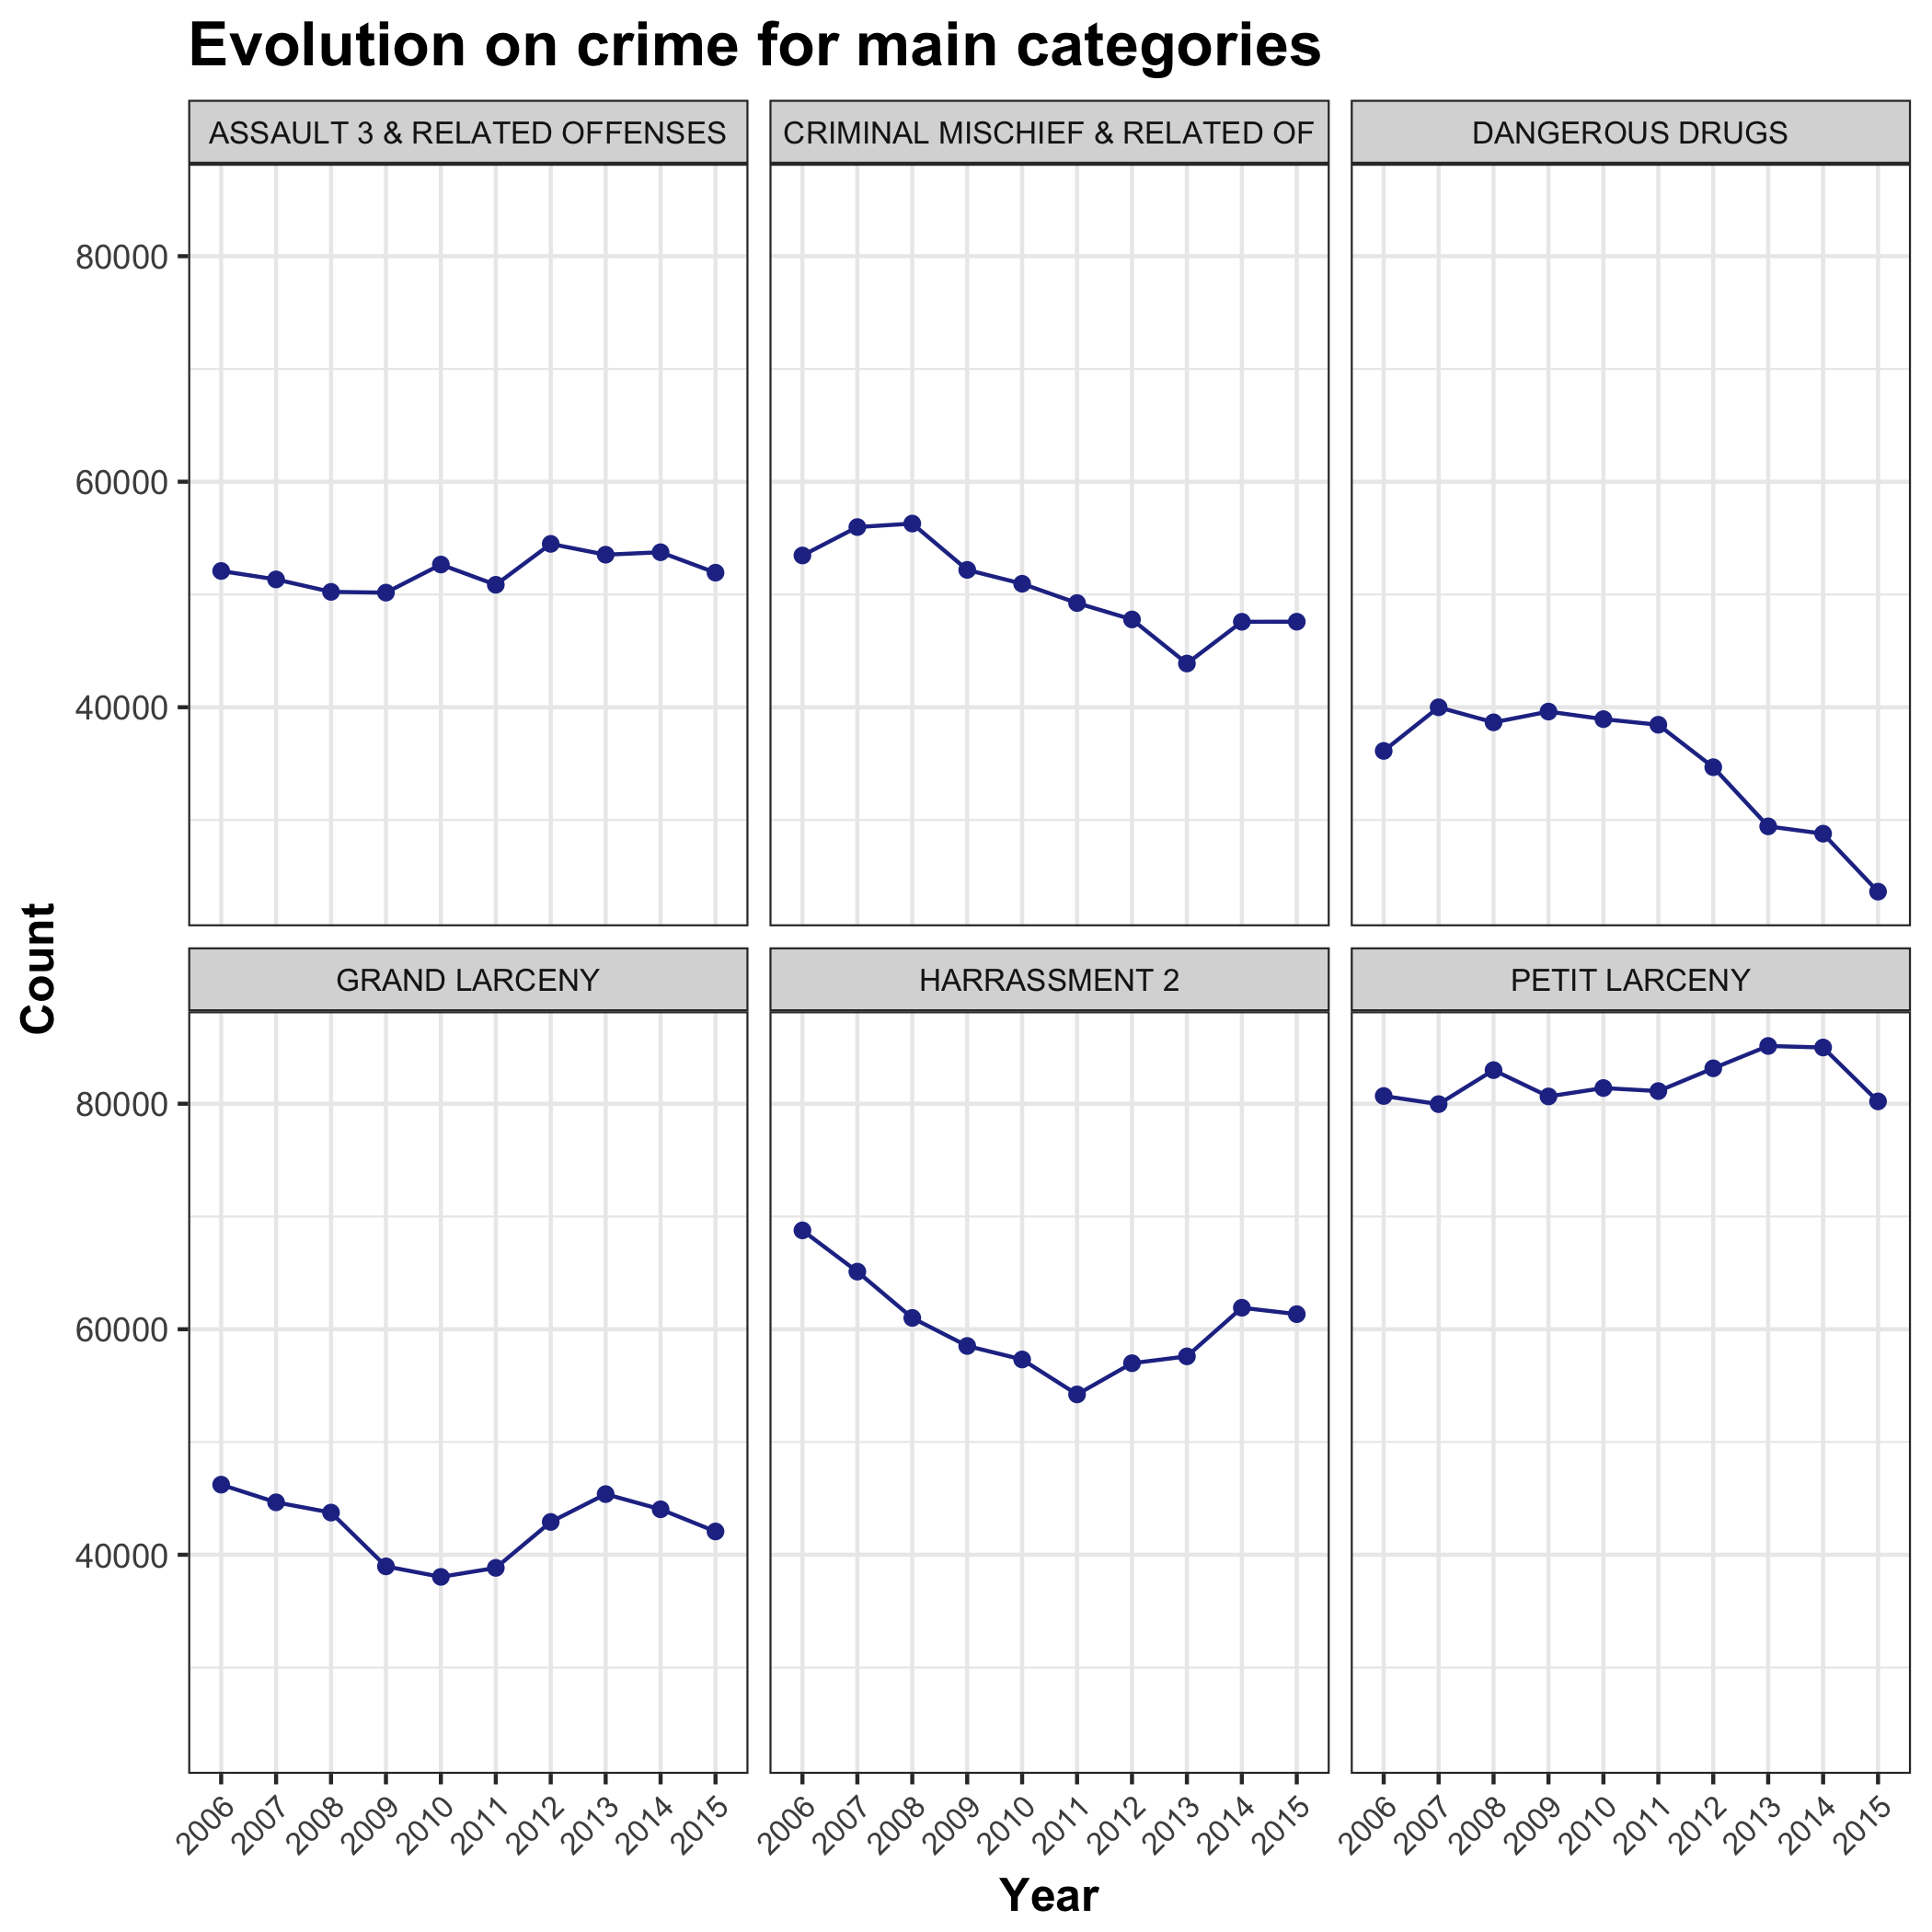
\includegraphics[scale=0.15]{7_MainCatsOverTime.png}
\end{figure}

\pagebreak
\section{Part II: TO BE DEFINED}


\begin{minted}{python}
[TO BE DEFINED]
\end{minted}



\newpage
\printbibliography 
\end{document}